\documentclass[pdflatex,sn-mathphys-num]{sn-jnl}

\usepackage[utf8]{inputenc}
\usepackage[T1]{fontenc}
\usepackage[spanish,es-tabla]{babel}
\usepackage{graphicx}
\usepackage{multirow}
\usepackage{amsmath,amssymb,amsfonts}
\usepackage{amsthm}
\usepackage{mathrsfs}
\usepackage[title]{appendix}
\usepackage{xcolor}
\usepackage{textcomp}
\usepackage{manyfoot}
\usepackage{booktabs}
\usepackage{tabularx}
\usepackage{array}
\usepackage{placeins}
\usepackage{hyperref}
\hypersetup{
  pdftitle={SM-CFHR: Regresor Huber Estructurado y Monotono en Factor de Capacidad para Pronostico Fotovoltaico Multi-Planta y Multi-Horizonte},
  pdfauthor={Jesus David Arevalo Montilla; Enmanuel David Diaz Molinares},
  pdfsubject={Pronostico fotovoltaico multi-planta y multi-horizonte},
  pdfkeywords={Pronostico fotovoltaico, Factor de capacidad, Perdida de Huber, Regularizacion estructurada, Restricciones de monotonia, Verificacion formal en Lean 4}
}

\renewcommand{\topfraction}{0.92}
\renewcommand{\bottomfraction}{0.85}
\renewcommand{\textfraction}{0.05}
\renewcommand{\floatpagefraction}{0.65}
\setcounter{topnumber}{4}
\setcounter{bottomnumber}{3}
\setcounter{totalnumber}{6}

\newcolumntype{L}{>{\raggedright\arraybackslash}X}
\newcolumntype{R}{>{\raggedleft\arraybackslash}X}

\theoremstyle{thmstyleone}
\newtheorem{theorem}{Teorema}
\newtheorem{proposition}{Proposición}
\newtheorem{lemma}{Lema}
\newtheorem{corollary}{Corolario}
\theoremstyle{thmstyletwo}
\newtheorem{remark}{Observación}
\theoremstyle{thmstylethree}
\newtheorem{definition}{Definición}

\DeclareMathOperator{\clip}{clip}
\DeclareMathOperator{\MAD}{MAD}
\DeclareMathOperator{\diag}{diag}
\DeclareMathOperator{\sign}{sign}

\raggedbottom

\begin{document}

\title[SM-CFHR para pronóstico fotovoltaico multihorizonte]{SM-CFHR: Regresor Huber Estructurado y Monótono en Factor de Capacidad para Pronóstico Fotovoltaico Multi-Planta y Multi-Horizonte}

\author[1]{\fnm{Jesús David} \sur{Arévalo Montilla}}\email{jdarevalo@uninorte.edu.co}
\author*[1]{\fnm{Enmanuel David} \sur{Diaz Molinares}}\email{denmanuel@uninorte.edu.co}

\affil*[1]{\orgdiv{Departamento de Matemáticas y Ciencia de Datos, Programa de Ciencia de Datos}, \orgname{Universidad del Norte}, \orgaddress{\city{Barranquilla}, \country{Colombia}}}

\abstract{El pronóstico determinístico diario ($D+1$) y subestacional ($7$--$28$~días) de generación fotovoltaica en flotas reales enfrenta heterogeneidad de escala cercana a $40\times$, episodios operativos atípicos y degradación de los pronósticos numéricos del tiempo (NWP) con el horizonte. Este trabajo formaliza, analiza matemáticamente, verifica en Lean~4 y evalúa fuera de muestra el estimador \textit{Structured Monotone Capacity-Factor Huber Regressor} (SM-CFHR) sobre $17$ centrales solares colombianas agrupadas en $7$ zonas espaciales ($2024$--$2026$; $9{,}8$--$388{,}0$~MW; $12\,725$ registros útiles). El modelo normaliza causalmente la energía diaria y acumulada por la capacidad máxima vigente al origen ($24\,000\,C_{i,t}$), escala la respuesta mediante mediana y MAD, y minimiza la pérdida de Huber bajo penalización $L_2$ diferenciada ($\alpha_{\mathrm{lin}}$ para dinámica/calendario; $\alpha_{\mathrm{meteo}}$ para variables NWP) y cotas no negativas sobre persistencia reciente e irradiación pronosticada, resuelta vía L-BFGS-B. Se demuestran convexidad global, regularidad $C^1$ con gradiente Lipschitz, existencia, unicidad de los pesos y condicional del intercepto, condiciones KKT, acotación de influencia en respuesta y monotonía parcial tras la proyección a $[0,1]$, respaldadas por $26$ declaraciones en Lean~4 sobre $\mathbb{R}$. En $28$ configuraciones fuera de muestra ($14\,625$ unidades por variante) comparando sistemas completos tal como fueron configurados frente a $22$ referencias en energía bruta, \texttt{SM-CFHR-Fixed} ($B=0$) alcanza rango medio $2{,}93/23$ en $\mathrm{MAE}_{\mathrm{macro}}$ ($\text{kWh}$, $18/28$ victorias descriptivas frente a \texttt{Mejor\_Bib}), $4{,}00/23$ en factor de capacidad adimensional ($\mathrm{MAE}_{\mathrm{CF,macro}}$, $16/28$ victorias) y supera a \texttt{SM-CFHR-HPO} ($B=25$) en $19/28$ escenarios con un coste de pared $59\times$ menor. En el análisis retrospectivo posterior (\texttt{v2.0.0}) sobre $\mathrm{MAE}_{\mathrm{macro}}$ con bloques disjuntos ($h_{\mathrm{serie}}=1$), se observan diferencias estadísticamente significativas tras Holm en los $5$ escenarios espaciotemporales con clima frente a \texttt{Mejor\_Bib} seleccionado \textit{ex post} ($p_{\mathrm{Holm}} \le 5{,}21\times 10^{-6}$, $T_{\mathrm{eff,macro}} \ge 30{,}82$) y en las $45/45$ comparaciones pareadas frente a las nueve bibliotecas ($p_{\mathrm{Holm,252}} \le 0{,}0417$), mientras en estrategia directa intraplanta sin clima el modelo pierde hasta $+24{,}24\%$. Dado que las $22$ referencias operaron en energía bruta ($\text{kWh}$) y la inferencia sobre la cohorte explorada es retrospectiva, no se declara superioridad algorítmica universal ni validación prospectiva independiente.}

\keywords{Pronóstico fotovoltaico, Factor de capacidad, Pérdida de Huber, Regularización estructurada, Restricciones de monotonía, Verificación formal en Lean~4}

\maketitle

\section{Introducción}\label{sec:intro}

La operación diaria y la programación subestacional de sistemas eléctricos hidrotérmicos con participación creciente de generación solar fotovoltaica (FV) requieren pronósticos determinísticos confiables desde el horizonte de un día ($D+1$) hasta cuatro semanas ($7$ a $28$ días). En el Sistema Interconectado Nacional (SIN) de Colombia, este problema plantea dos exigencias simultáneas: anticipar la producción de centrales individuales con historial propio y estimar la generación de emplazamientos o zonas geográficas nuevas a partir de plantas de referencia. En ambos casos, la capacidad nominal instalada resume el tamaño de la planta bajo condiciones estándar de ensayo, pero resulta insuficiente para predecir la energía entregada, pues la irradiancia incidente, la temperatura de celda, la nubosidad convectiva tropical, la relación DC/AC, las ampliaciones escalonadas de potencia neta y las restricciones operativas separan la producción observada de la capacidad teórica de placa \cite{mueller2016yield,trigo2021models,purohit2018performance}.

Cuando se modela una flota heterogénea en lugar de una sola instalación, la formulación directa en unidades de energía bruta ($\text{kWh/día}$) introduce una distorsión estructural inmediata. En la cohorte analizada en este estudio ---$17$ plantas reales del mercado eléctrico colombiano entre enero de 2024 y octubre de 2026--- la capacidad efectiva neta varía entre $9{,}8$~MW y $388{,}0$~MW, lo que representa un cociente de escala de $39{,}6\times$. Bajo una función de pérdida calculada en $\text{kWh}$ sin normalización previa, los residuos de una central de gran escala dominan el gradiente frente a los de plantas pequeñas, impidiendo transferir parámetros entre zonas geográficas. Al mismo tiempo, los registros operativos reales contienen colas asimétricas hacia cero ocasionadas por días incompletos, desconexiones parciales, nubosidad severa o restricciones operativas, frente a los cuales la pérdida cuadrática ordinaria resulta excesivamente sensible, y los pronósticos numéricos del tiempo (NWP) pierden habilidad predictiva conforme el horizonte se extiende hacia dos, tres y cuatro semanas.

Frente a estas dificultades, este trabajo formaliza, analiza y establece el protocolo de evaluación del modelo \textit{Structured Monotone Capacity-Factor Huber Regressor} (\textbf{SM-CFHR}). El estimador responde a una secuencia de decisiones constructivas motivadas por los datos: normaliza tanto los niveles históricos recientes como la variable objetivo al espacio adimensional del factor de capacidad mediante la energía nominal máxima vigente al origen de predicción, $24\,000\,C_{i,t}$; estabiliza la respuesta frente a episodios anómalos estandarizándola con mediana y desviación absoluta mediana (MAD) estimadas exclusivamente en entrenamiento, y minimiza una pérdida de Huber \cite{huber1964,huber2009robust}; introduce una penalización cuadrática diferenciada entre dinámica temporal/calendario ($\alpha_{\mathrm{lin}}$) y variables meteorológicas ($\alpha_{\mathrm{meteo}}$); e impone restricciones de no negatividad sobre los coeficientes de persistencia de treinta días y de irradiación horizontal pronosticada, resolviendo el programa convexo resultante mediante L-BFGS-B con gradiente analítico exacto \cite{byrd1995lbfgsb,zhu1997lbfgsb}.

Dado que la arquitectura de SM-CFHR se fijó tras inspeccionar el comportamiento del panel histórico 2024--2026, la evaluación fuera de muestra (OOF) sobre ese mismo periodo debe interpretarse bajo la advertencia de reutilización adaptativa \cite{cawley2010overfit} y no equivale a una muestra confirmatoria prospectiva independiente.

Las contribuciones verificables del trabajo son tres: (1) la formulación de SM-CFHR basada en normalización causal por capacidad vigente ($24\,000\,C_{i,t}$), regularización anisotrópica y restricciones de monotonía integrada en un protocolo multihorizonte sin fuga; (2) el análisis convexo y verificación formal en Lean~4 de sus propiedades sobre $\mathbb{R}$; y (3) la evaluación fuera de muestra en $28$ configuraciones experimentales frente a $22$ referencias en energía bruta, junto con la reconciliación inferencial sobre $\mathrm{MAE}_{\mathrm{macro}}$ y $\mathrm{MAE}_{\mathrm{CF,macro}}$ que delimita la ventaja confirmada al régimen espaciotemporal con meteorología y documenta explícitamente sus derrotas en estrategia directa intraplanta sin clima.

\section{Fundamentos y estado del arte}\label{sec:estado}

\subsection{Pronóstico fotovoltaico operacional, heterogeneidad y normalización física}

La brecha entre el rendimiento teórico de placa y la energía medida en centrales conectadas a red constituye un fenómeno bien documentado en la literatura empírica. Müller et~al.~\cite{mueller2016yield} contrastaron estimaciones de rendimiento frente a mediciones reales de $26$ plantas en Alemania y España, mostrando que los sesgos en bases de irradiación y las pérdidas operativas generan desviaciones sistemáticas; Purohit y Purohit~\cite{purohit2018performance} observaron discrepancias análogas en centrales de la India. Al extender el análisis desde instalaciones aisladas hacia flotas heterogéneas o modelos transferibles entre emplazamientos, Trigo-González et~al.~\cite{trigo2019hourly,trigo2021models} formularon regresiones lineales múltiples y modelos no lineales sobre el \textit{Performance Ratio} en Chile y España bajo pérdida cuadrática, mientras que Lehmann et~al.~\cite{lehmann2023benchmark} compararon ocho soluciones comerciales intradía. En el contexto colombiano, Pico et~al.~\cite{pico2026shortterm} evaluaron algoritmos de aprendizaje automático a resolución de diez minutos para el horizonte de un día sobre $7$ plantas; sin embargo, emplearon potencia simulada mediante SAM/NSRDB y partición puramente cronológica, sin generación real medida por el operador del mercado ni horizontes subestacionales.

Para comparar de manera coherente centrales cuya capacidad instalada difiere en órdenes de magnitud, Yang et~al.~\cite{yang2020} sistematizaron buenas prácticas de verificación determinística solar, recomendando normalizar las métricas por capacidad instalada o cielo despejado, reportar \textit{skill scores} frente a referencias causales ingenuas y preservar la no anticipación temporal al procesar salidas numéricas del tiempo (NWP). Esta recomendación motiva directamente la normalización causal de SM-CFHR por $24\,000\,C_{i,t}$: mientras la literatura suele normalizar únicamente las métricas finales de evaluación, en flotas con $39{,}6\times$ de diferencia de escala y ampliaciones escalonadas de potencia es igualmente necesario normalizar la variable objetivo y los predictores históricos antes de optimizar la función de pérdida.

\subsection{Pronósticos diarios, subestacionales y posprocesamiento meteorológico}

En horizontes cortos ($D+1$), los pronósticos NWP presentan sesgos locales sistemáticos debidos a topografía, nubosidad convectiva subgrilla y parametrización atmosférica. Glahn y Lowry~\cite{glahn1972mos} introdujeron el posprocesamiento estadístico (\textit{Model Output Statistics}, MOS) para corregir salidas numéricas mediante regresión sobre observaciones locales; posteriormente, Bacher et~al.~\cite{bacher2009online} acoplaron predicciones NWP con dinámica autorregresiva reciente en generación solar en línea, y Yang y van der Meer~\cite{yang2021postprocessing} sintetizaron los principios modernos del posprocesamiento solar. Al extender la predicción hacia horizontes subestacionales de una a cuatro semanas, la señal determinística de los ensambles NWP se degrada progresivamente: Bloomfield et~al.~\cite{bloomfield2021} mostraron en $28$ países europeos que las anomalías meteorológicas calibradas aportan habilidad en las primeras dos semanas antes de converger hacia la climatología reciente. No obstante, sigue abierto en qué medida una penalización $L_2$ diferenciada sobre las variables NWP logra retener señal útil a $14$--$28$ días en regiones tropicales sin sobreajustar errores de mediano plazo.

\subsection{Estimación robusta, regularización anisotrópica y restricciones de caja}

Los registros operativos de energía eléctrica exhiben colas asimétricas por fallas de telemetría, días incompletos y restricciones operativas. Huber~\cite{huber1964} formuló los estimadores $M$ con pérdida cuadrático-lineal como solución minimax frente a contaminación en la vecindad de la normal, y Huber y Ronchetti~\cite{huber2009robust} desarrollaron su teoría asintótica. Sin embargo, como demostraron Hampel et~al.~\cite{hampel1986robust} mediante la teoría de la función de influencia, la pérdida de Huber acota la sensibilidad frente a valores atípicos en la variable respuesta, pero \emph{no} protege frente a puntos de apalancamiento arbitrarios en el espacio de covariables (a diferencia de estimadores de tipo Mallows o Schweppe). Para estabilizar la escala frente a colas pesadas en la respuesta, la desviación absoluta mediana (MAD) proporciona un estimador robusto con punto de ruptura del $50\%$ \cite{rousseeuw1993mad}.

En el plano de la regularización, la penalización cuadrática clásica de Hoerl y Kennard~\cite{hoerl1970} y la selección $L_1$ de Tibshirani~\cite{tibshirani1996} fueron combinadas con pérdidas robustas de Huber por Owen~\cite{owen2007}, quien estudió su estructura convexa bajo colinealidad. Por su parte, la teoría general de optimización convexa \cite{boyd2004convex} establece que imponer restricciones simples de signo sobre subconjuntos de parámetros mantiene el problema dentro de un poliedro cerrado y convexo, permitiendo su resolución mediante el algoritmo cuasi-Newton L-BFGS-B \cite{byrd1995lbfgsb,zhu1997lbfgsb} disponible en SciPy \cite{virtanen2020scipy} sin requerir derivadas segundas continuas.

\subsection{Estrategias multihorizonte, alternativas comparadas y evaluación espaciotemporal}

El pronóstico a varios días enfrenta un compromiso clásico entre estrategias recursivas y directas \cite{bentaieb2012,chevillon2007}: la vía recursiva entrena un modelo de un paso y realimenta sus propias predicciones, acumulando error cuando la dinámica presenta deriva; la vía directa ajusta modelos específicos por horizonte, evitando la propagación recursiva a costa de ignorar correlaciones entre pasos intermedios.

Para contrastar si la formulación paramétrica de SM-CFHR aporta ventajas reales frente a enfoques alternativos, el estudio compara dos familias consolidadas de competidores además de la línea base causal de media móvil de $30$ días (\texttt{MM30}):
\begin{enumerate}
    \item \textbf{Estimadores estándar de biblioteca ($9$ modelos):} implementados en \texttt{scikit-learn} \cite{pedregosa2011sklearn} y \texttt{xgboost} directamente sobre energía diaria en $\text{kWh/día}$: regresores lineales regularizados (\texttt{Ridge} \cite{hoerl1970}, \texttt{Lasso} \cite{tibshirani1996}, \texttt{BayesianRidge} \cite{mackay1992}), máquinas de vectores de soporte (\texttt{SVR} \cite{drucker1997svr}), vecinos más cercanos (\texttt{k-NN} \cite{cover1967nearest}) y modelos de árboles y ensambles (\texttt{DecisionTree} \cite{breiman1984cart}, \texttt{Random Forest} \cite{breiman2001}, \texttt{HistGradientBoosting} \cite{friedman2001gbm} y \texttt{XGBoost} \cite{chen2016}). Esta familia evalúa la capacidad de regresores flexibles sin normalización de escala.
    \item \textbf{Adaptaciones residuales específicas del dominio ($12$ modelos):} implementaciones propias del proyecto que modelan el residuo estandarizado respecto al nivel reciente en $\text{kWh/día}$, permitiendo aislar el efecto de la arquitectura frente a distintas técnicas estadísticas clásicas: regresión Ridge residual (\texttt{RLAC} \cite{hoerl1970}), regresión local ponderada por distancia y planta/grupo (\texttt{IWLAR}, inspirada en \cite{cleveland1979robust,atkeson1997locally}), mezcla convexa fija entre Ridge y Huber (\texttt{WCFC}, basada en \cite{bates1969combination,huber1964,hoerl1970}), proceso gaussiano con núcleo RBF sobre submuestra estratificada (\texttt{ABGPR} \cite{rasmussen2006gpml}), regresión Ridge jerárquica cerrada con efectos por grupo/planta e interacción radiativa (\texttt{HARC}, inspirada en \cite{laird1982random,hoerl1970}), corrección reciente de sesgo tipo MOS en ventana móvil (\texttt{SRMOS} \cite{glahn1972mos}), nivel por suavizamiento exponencial (\texttt{ELAC} \cite{brown1959statistical}) o filtro de Kalman escalar (\texttt{KLAC} \cite{kalman1960approach,harvey1989forecasting}), regresión de Huber residual en $\text{kWh}$ (\texttt{RARC} \cite{huber1964}), bosques cuantílicos sobre residuos en hojas (\texttt{RQRF} \cite{koenker1978quantiles,meinshausen2006}), descomposición de desviación lineal (\texttt{PDEC} \cite{hyndman2021fpp3,hoerl1970}) y gradient boosting residual (\texttt{MARB} \cite{chen2016}). Estas doce variantes constituyen adaptaciones propias para el experimento comparativo y no deben confundirse con reproducciones exactas de paquetes externos.
\end{enumerate}

En materia de evaluación, la partición aleatoria por filas en paneles espaciotemporales sobreestima la capacidad predictiva \cite{roberts2017crossvalidation}. Prevenir la fuga de datos exige estimar toda imputación, estandarización e hiperparámetros dentro del entrenamiento \cite{kaufman2012leakage,tashman2000,cerqueira2020}, recurriendo a validación cruzada anidada \cite{varma2006bias,cawley2010overfit} y optimización bayesiana TPE \cite{bergstra2011tpe,akiba2019optuna}. Asimismo, la inferencia sobre series dependientes requiere contrastes calibrados ante autocorrelación y multiplicidad \cite{diebold1995,harvey1997,newey1987,giacomini2006tests,clark2007nested,hansen2005spa,hansen2011mcs,politis1994stationary,holm1979,benjamini1995fdr,cliff1993dominance}, manteniendo cautela con pocos conglomerados espaciales \cite{cameron2015cluster}, e intervalos conformes temporales sin supuestos gaussianos \cite{vovk2005conformal,lei2018conformal,barber2023nonexchangeable}.

\subsection{Delimitación de teoría establecida y contribuciones del trabajo}

Para evitar ambigüedades sobre el alcance de la originalidad científica, distinguimos seis niveles:
\begin{enumerate}
    \item \textbf{Conocimiento matemático y estadístico establecido:} la convexidad y condiciones KKT de programas poliedrales \cite{boyd2004convex}, la función de influencia acotada en respuesta y no acotada en apalancamiento de Huber \cite{huber1964,hampel1986robust,huber2009robust}, la consistencia del escalado MAD \cite{rousseeuw1993mad} y la convergencia estacionaria de L-BFGS-B \cite{byrd1995lbfgsb,zhu1997lbfgsb}.
    \item \textbf{Métodos publicados utilizados o adaptados:} L-BFGS-B vía SciPy, optimización TPE vía Optuna, pruebas DM--HLN--HAC, MCS, SPA, GW, CW, predicción conforme dividida y los $9$ estimadores estándar de biblioteca.
    \item \textbf{Decisiones de modelado propias:} la integración específica en SM-CFHR de normalización causal al origen por $24\,000\,C_{i,t}$, escalado MAD de la respuesta, regularización $L_2$ anisotrópica entre dinámica temporal y variables NWP, cotas de no negatividad sobre persistencia e irradiación y despliegue recursivo causal exacto con amortiguamiento geométrico.
    \item \textbf{Resultados matemáticos específicos demostrados para SM-CFHR:} las condiciones precisas de coercividad y existencia con intercepto no penalizado ($n \ge 1$, $\alpha_{\mathrm{lin}}, \alpha_{\mathrm{meteo}} > 0$), la unicidad global de $\mathbf{w}^*$ frente a la unicidad meramente condicional de $b^*$ (junto con el contraejemplo explícito $n=2$), las cotas exactas por observación al gradiente y la monotonía parcial \textit{ceteris paribus} tras el truncamiento físico en $[0,1]$.
    \item \textbf{Verificación formal en Lean~4:} la comprobación mecánica en Lean~4 \cite{moura2021lean4} y Mathlib \cite{mathlib2020} de los enunciados anteriores sobre $\mathbb{R}$, lo cual valida la consistencia lógica de las pruebas sin constituir un descubrimiento matemático nuevo ni verificar el código Python.
    \item \textbf{Contribuciones empíricas pendientes:} el desempeño comparativo en las $28$ configuraciones experimentales y las hipótesis H1--H4 permanecen abiertas a la finalización de la ejecución OOF en curso.
\end{enumerate}

\section{Datos, depuración de cohorte y análisis exploratorio}\label{sec:datos_eda}

Antes de formular los conjuntos experimentales o el estimador, esta sección caracteriza las fuentes de datos, las reglas de depuración física con sus posibles sesgos de selección, y la evidencia exploratoria que motiva cada decisión de modelado.

\subsection{Fuentes de información y depuración causal de la cohorte}

La base empírica cubre el periodo comprendido entre el 1 de enero de 2024 y el 31 de octubre de 2026 ($1\,035$ días calendario) e integra cuatro fuentes auditadas: (1) generación horaria real medida y capacidad efectiva neta diaria reportadas por el operador del mercado eléctrico colombiano XM \cite{xm2026api}; (2) coordenadas geográficas verificadas de las centrales en el \textit{Global Solar Power Tracker} \cite{gem2026solar}; (3) pronósticos meteorológicos horarios a $24\text{ h}$ de antelación (promedio del ensamble ECMWF IFS $0{,}25^\circ$, GFS e ICON) recuperados de los archivos históricos de la API \textit{Previous Runs} de Open-Meteo \cite{openmeteoPreviousRuns}; y (4) corridas operacionales subestacionales del sistema NOAA GEFSv12 (\texttt{00~UTC}, pasos horarios hasta $696\text{ h}$, equivalentes a $29$ días), totalizando $65\,688$ registros completos planta--origen--horizonte. Durante la auditoría inicial se descartó reconstruir pronósticos históricos $D+1$ a partir de las primeras horas de las corridas de archivo, pues su elevada proximidad al reanálisis meteorológico (correlación $0{,}976$ frente a $0{,}615$ del pronóstico real emitido con $24\text{ h}$ de antelación) habría introducido fuga de información futura.

El protocolo de depuración física \cite{nist2003eda,pipino2002quality,jensen2024solarqc} parte de $30\,964$ registros recurso--día de XM y aplica filtros secuenciales estrictos: existencia de capacidad efectiva neta registrada en la fecha, generación y capacidad estrictamente positivas, plausibilidad física $\mathrm{cf}^{\mathrm{obs}}_{i,t} \le 1{,}05$ (admitiendo un margen de $5\%$ para tolerar pequeñas diferencias horarias antes de reportar ampliaciones), coordenadas verificadas, al menos $60$ días transcurridos desde la entrada en operación comercial y un mínimo de $100$ días útiles por planta. La Figura~\ref{fig:cohorte_mapa} resume el flujo cuantitativo de depuración hasta consolidar $12\,756$ observaciones planta--día en $M=17$ centrales distribuidas en $G=7$ zonas geográficas (agrupadas por enlace simple a menos de $100\text{ km}$). Para el ajuste y evaluación causal se exige además contar con más de $6$ horas reportadas en el día, excluyendo $31$ registros incompletos ($0{,}24\%$, todos con factor de capacidad inferior a $0{,}04$) hasta obtener $12\,725$ días válidos, sin imputar jamás la variable objetivo.

\begin{figure}[!htbp]
\centering
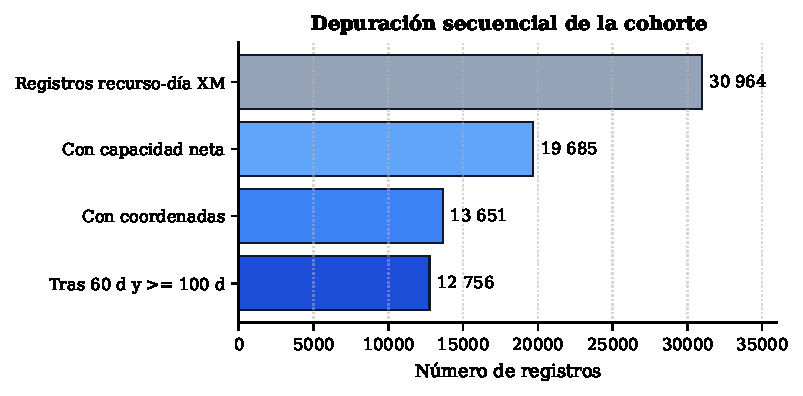
\includegraphics[width=0.86\textwidth]{figures/eda_flujo_cohorte.pdf}\\[0.5em]
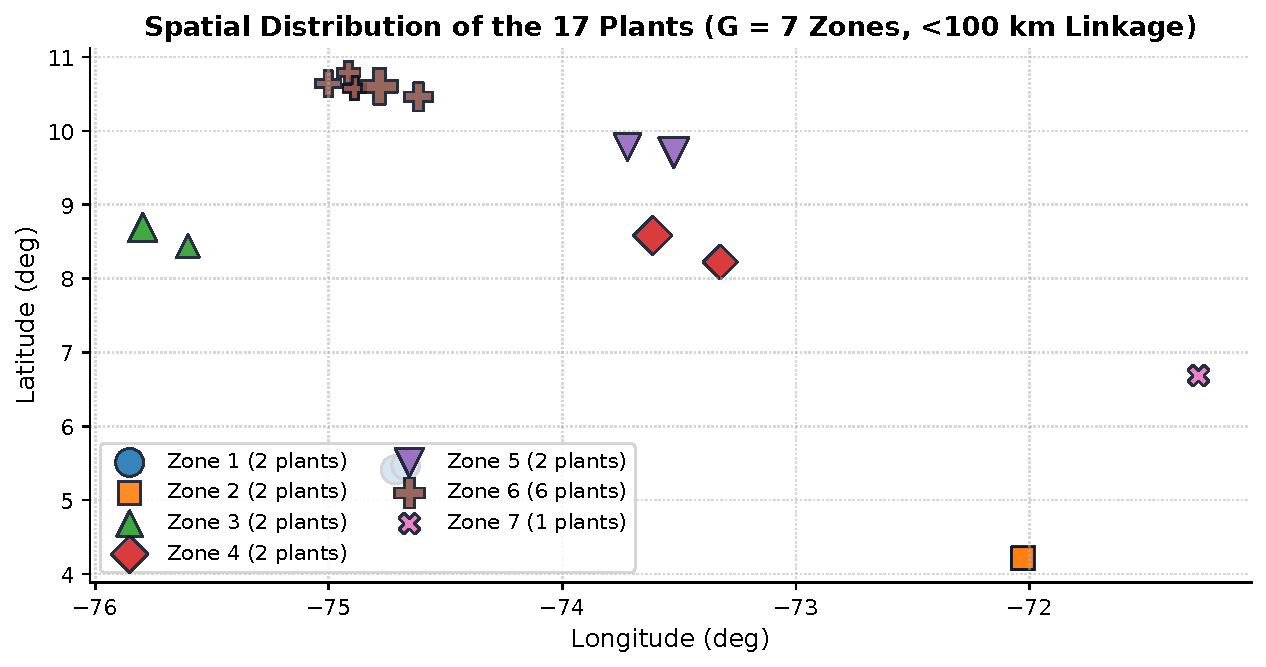
\includegraphics[width=0.86\textwidth]{figures/eda_mapa_plantas.pdf}
\caption{Depuración cuantitativa de la cohorte ($30\,964 \to 12\,756$ registros planta--día en $17$ centrales; arriba) y distribución geográfica en $G=7$ zonas espaciales por enlace simple a $<100\text{ km}$ (abajo).}
\label{fig:cohorte_mapa}
\end{figure}

Es indispensable explicitar los posibles sesgos de selección derivados de estos filtros: al excluir días con generación nula o $\le 6$ horas reportadas, las métricas reflejan operación activa o parcialmente activa y omiten paradas totales prolongadas; asimismo, el requisito de $\ge 100$ días útiles y $\ge 60$ días post-arranque excluye plantas recién conectadas en fase temprana de pruebas, concentrando la muestra en centrales operativamente estabilizadas cuya cobertura oscila entre $251$ y $1\,032$ días válidos (Tabla~\ref{tab:flota17}).

\begin{table}[!htbp]
\caption{Caracterización de las $17$ centrales fotovoltaicas de la cohorte (ordenadas por grupo espacial).}\label{tab:flota17}
\scriptsize
\setlength{\tabcolsep}{3.5pt}
\begin{tabular}{@{}clrrrrrr@{}}
\toprule
Cód. & Planta & Gr. & $n$ total & Cap.\ mín--máx (MW) & Inicio & Fin & Lat / Lon ($^\circ$) \\
\midrule
\texttt{3IRX} & Portón del Sol & 1 & 884 & $102{,}0$--$102{,}0$ & 2024-05-07 & 2026-10-31 & $5{,}41 / -74{,}71$ \\
\texttt{TPUY} & Parque Solar Tepuy & 1 & 812 & $83{,}0$--$100{,}0$ & 2024-08-11 & 2026-10-31 & $5{,}47 / -74{,}67$ \\
\texttt{3EDL} & Bosques Llanos V & 2 & 1\,034 & $17{,}9$--$17{,}9$ & 2024-01-01 & 2026-10-31 & $4{,}21 / -72{,}03$ \\
\texttt{3EFY} & Bosques Llanos IV & 2 & 1\,034 & $19{,}9$--$19{,}9$ & 2024-01-01 & 2026-10-31 & $4{,}22 / -72{,}03$ \\
\texttt{3IZ6} & Parque Solar La Unión & 3 & 805 & $100{,}0$--$102{,}0$ & 2024-08-18 & 2026-10-31 & $8{,}69 / -75{,}80$ \\
\texttt{3J2B} & Solar Planeta Rica & 3 & 868 & $19{,}9$--$19{,}9$ & 2024-06-16 & 2026-10-31 & $8{,}44 / -75{,}60$ \\
\texttt{3IQA} & Sunnorte & 4 & 643 & $35{,}0$--$35{,}0$ & 2025-01-25 & 2026-10-31 & $8{,}22 / -73{,}32$ \\
\texttt{MATA} & La Mata & 4 & 796 & $80{,}0$--$83{,}0$ & 2024-08-26 & 2026-10-31 & $8{,}59 / -73{,}61$ \\
\texttt{3DDT} & Latam Solar La Loma & 5 & 795 & $150{,}0$--$150{,}0$ & 2024-08-23 & 2026-10-31 & $9{,}71 / -73{,}52$ \\
\texttt{EPFV} & El Paso & 5 & 892 & $68{,}0$--$70{,}0$ & 2024-05-22 & 2026-10-31 & $9{,}78 / -73{,}72$ \\
\texttt{3HF5} & Fundación & 6 & 800 & $90{,}0$--$100{,}0$ & 2024-08-21 & 2026-10-31 & $10{,}46 / -74{,}62$ \\
\texttt{3INX} & Caracolí I & 6 & 618 & $50{,}0$--$50{,}0$ & 2025-02-20 & 2026-10-31 & $10{,}64 / -75{,}00$ \\
\texttt{3K8C} & BSB 503 & 6 & 699 & $19{,}9$--$19{,}9$ & 2024-11-25 & 2026-10-31 & $10{,}57 / -74{,}89$ \\
\texttt{3K8E} & BSB 504 & 6 & 698 & $19{,}9$--$19{,}9$ & 2024-11-26 & 2026-10-31 & $10{,}58 / -74{,}89$ \\
\texttt{4RGG} & Parque Solar Baranoa & 6 & 490 & $19{,}9$--$19{,}9$ & 2025-06-29 & 2026-10-31 & $10{,}79 / -74{,}92$ \\
\texttt{GYPO} & Guayepo & 6 & 635 & $370{,}0$--$388{,}0$ & 2025-01-29 & 2026-10-31 & $10{,}61 / -74{,}78$ \\
\texttt{5F43} & Alma II & 7 & 253 & $9{,}8$--$9{,}8$ & 2026-02-21 & 2026-10-31 & $6{,}69 / -71{,}28$ \\
\botrule
\end{tabular}
\end{table}

\subsection{Hallazgos exploratorios y su vínculo con el diseño del estimador}

Cada figura exploratoria responde una pregunta científica específica que condiciona las decisiones metodológicas posteriores:

\paragraph{1. ¿Qué heterogeneidad de cobertura, escala y ampliaciones presenta la flota?}
La Tabla~\ref{tab:flota17} y la Figura~\ref{fig:eda_cob_horas} muestran que las centrales entran en operación de forma escalonada (desde enero de 2024 hasta febrero de 2026), con capacidades netas entre $9{,}8$~MW (\texttt{5F43}) y $388{,}0$~MW (\texttt{GYPO}), un cociente de escala de $39{,}6\times$, y $7$ ampliaciones discretas de potencia neta en $6$ centrales (por ejemplo, \texttt{TPUY} de $83$ a $100$~MW y \texttt{3HF5} de $90$ a $100$~MW). Asimismo, la distribución de horas reportadas confirma la presencia de $31$ jornadas truncadas ($\le 6\text{ h}$) asociadas a valores anormalmente bajos. Estas dos observaciones justifican tres decisiones: (a) normalizar tanto predictores históricos como objetivos en factor de capacidad usando exclusivamente la capacidad vigente al origen $C_{i,t}$ sin anticipar ampliaciones futuras; (b) agregar errores mediante macro-promedio por planta ($\mathrm{MAE}_{\mathrm{macro}}$) para no quedar dominados por las plantas de mayor potencia o mayor longitud de serie; y (c) excluir días incompletos de $\le 6\text{ h}$ para no contaminar la señal física con fallas de telemetría.

\begin{figure}[!htbp]
\centering
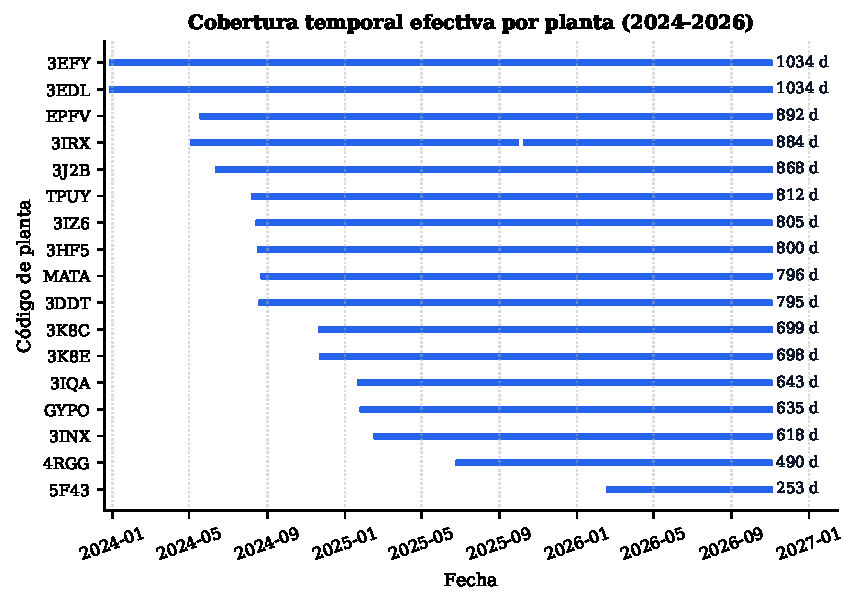
\includegraphics[width=0.92\textwidth]{figures/eda_cobertura_temporal.pdf}\\[0.5em]
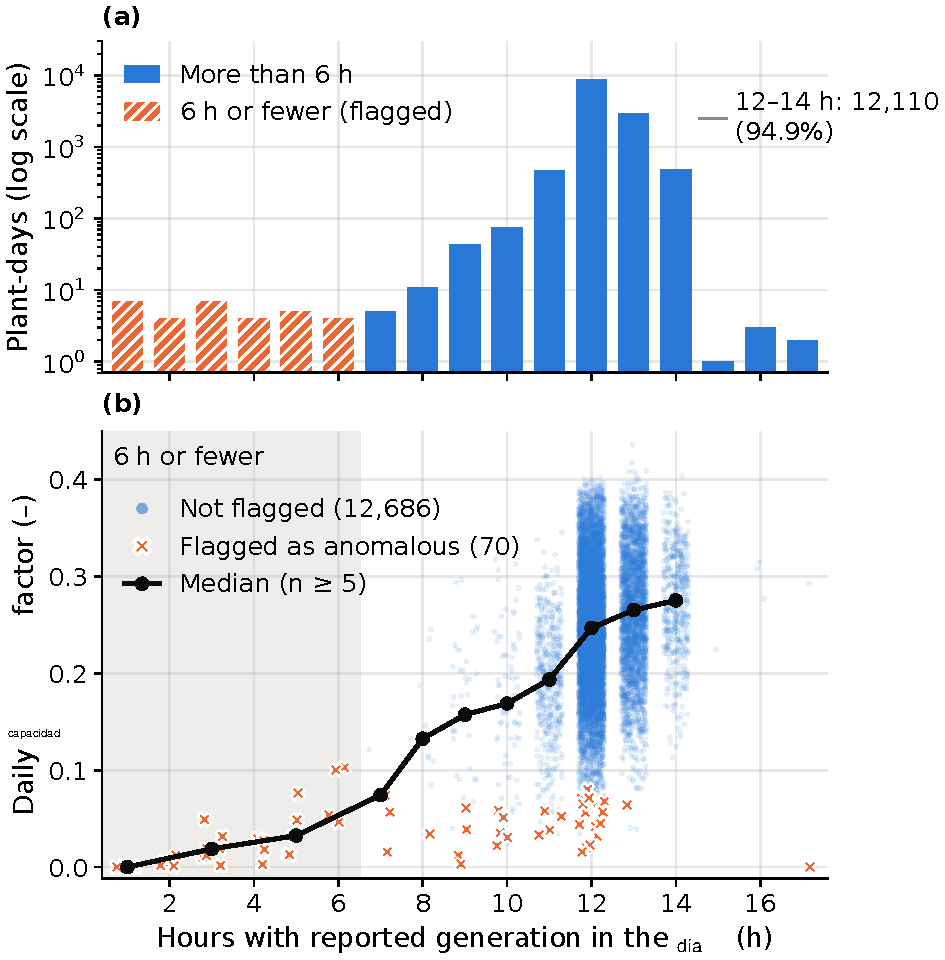
\includegraphics[width=0.92\textwidth]{figures/eda_horas_y_anomalos.pdf}
\caption{Cobertura temporal heterogénea por planta ($251$ a $1\,032$ días útiles; arriba) y distribución de horas reportadas por XM mostrando los registros incompletos excluidos ($\le 6\text{ h}$; abajo).}
\label{fig:eda_cob_horas}
\end{figure}

\paragraph{2. ¿Cómo se distribuyen el factor de capacidad y la relación con la irradiación?}
La Figura~\ref{fig:eda_univ} muestra que el factor de capacidad diario observado posee media $0{,}248$, mediana $0{,}250$ (rango intercuartílico $0{,}203$--$0{,}295$; máximo $0{,}436$) y una cola izquierda extendida hacia cero. Al graficarlo frente a la irradiación horizontal diaria pronosticada, se observa una asociación positiva monótona acompañada de $68$ episodios de rendimiento específico reducido (cociente entre factor de capacidad normalizado e irradiación inferior a $0{,}3$). Sin registros independientes de consignas de despacho no puede atribuirse la totalidad de esos episodios a \textit{curtailment}: reflejan una mezcla de restricciones operativas, desconexiones parciales, mantenimiento y nubosidad convectiva local no capturada por la malla NWP. Desde el punto de vista metodológico, esta evidencia motiva evaluar la pérdida de Huber con escalado robusto MAD para acotar el peso de caídas anómalas en la respuesta, junto con restricciones de signo no negativo sobre la irradiación pronosticada y la persistencia reciente para evitar pendientes negativas espurias.

\begin{figure}[!htbp]
\centering
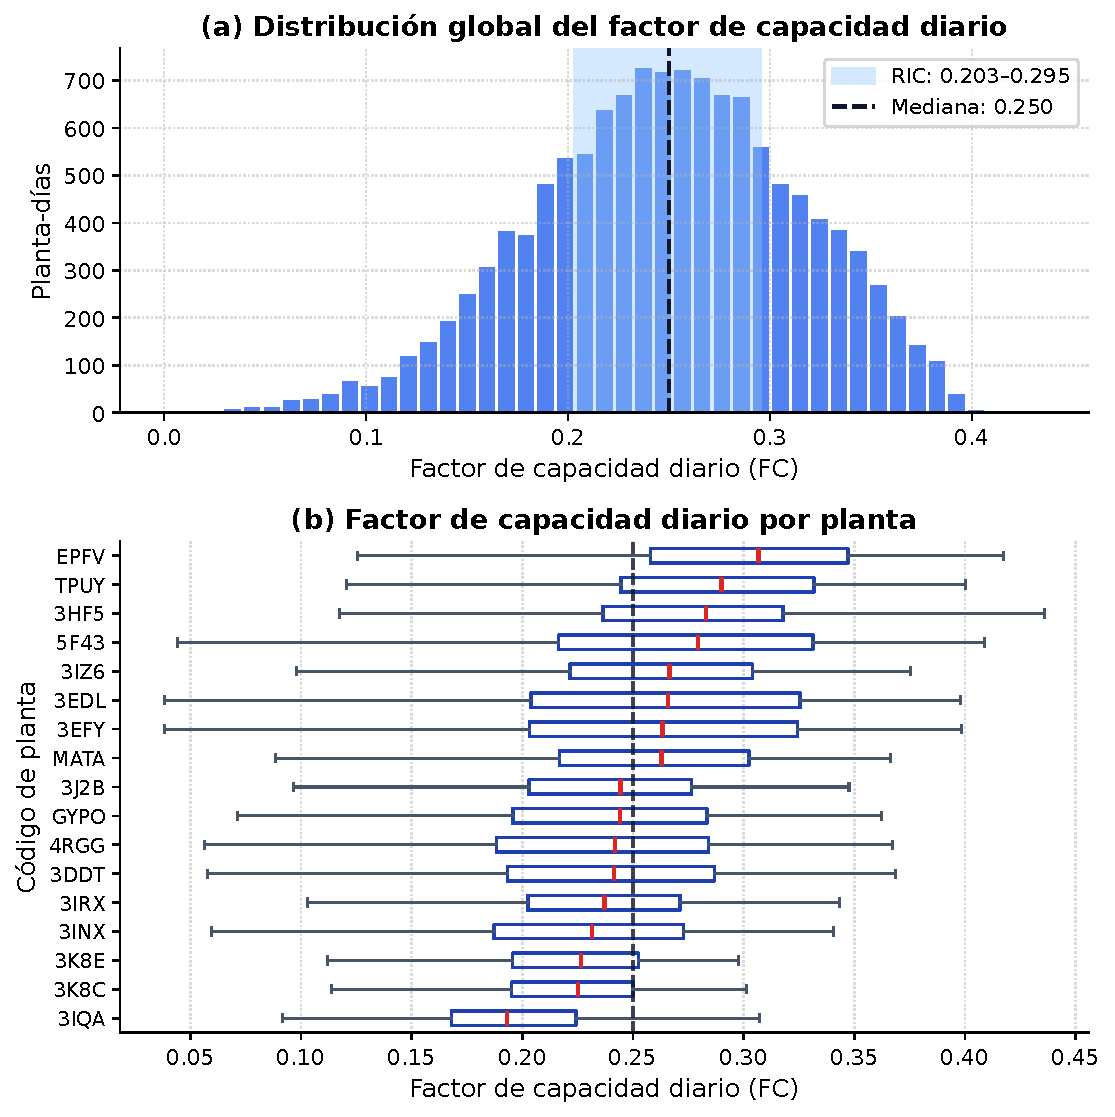
\includegraphics[width=0.49\textwidth]{figures/eda_distribucion_fc.pdf}
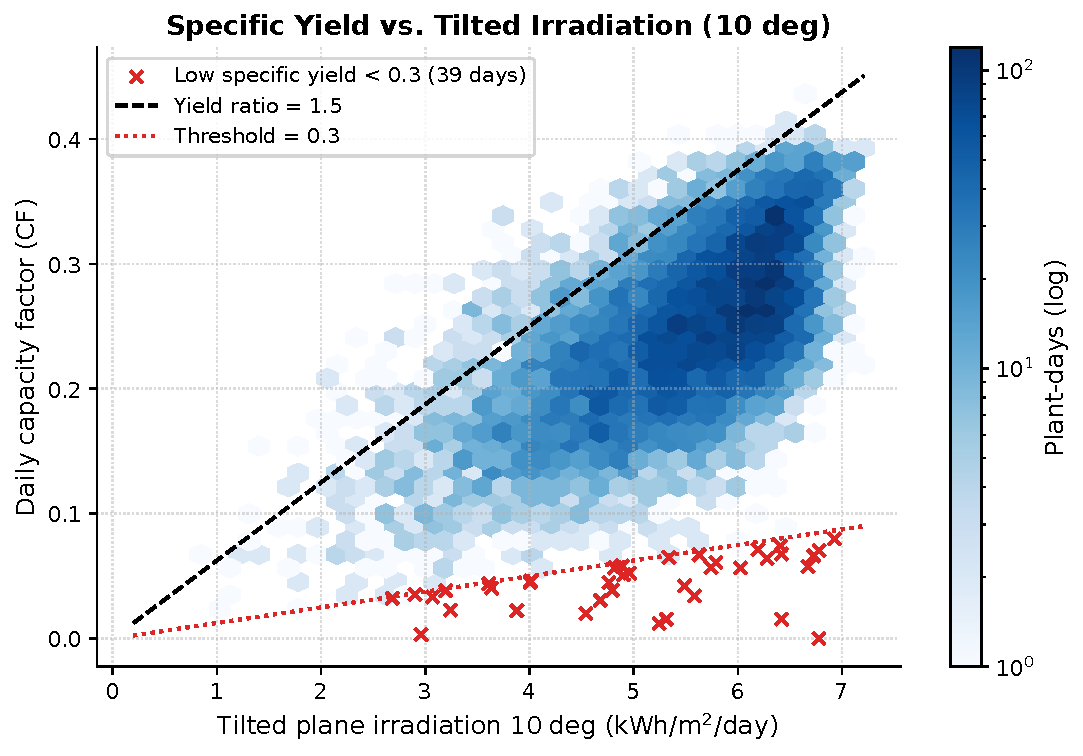
\includegraphics[width=0.49\textwidth]{figures/eda_rendimiento_especifico.pdf}
\caption{Distribución asimétrica del factor de capacidad diario observado (izquierda) y relación empírica frente a la irradiación diaria destacando $68$ episodios de rendimiento específico reducido (derecha).}
\label{fig:eda_univ}
\end{figure}

\paragraph{3. ¿Qué estructura de estacionalidad, persistencia y acoplamiento espacial existe?}
La Figura~\ref{fig:eda_est_dep} evidencia una variación mensual moderada acorde con los ciclos climáticos de Colombia (regiones Caribe, Andina y Orinoquía), una autocorrelación positiva pronunciada en rezagos cortos que decae progresivamente con el tiempo, y correlaciones cruzadas significativas entre plantas pertenecientes a la misma zona geográfica ($<100\text{ km}$). La persistencia temporal fundamenta incluir medias móviles causales de $30$ y $7$ días junto con diferencias amortiguadas por horizonte y armónicos anuales de calendario; a su vez, la elevada correlación intrazonal demuestra que una validación espacial ingenua por planta individual filtraría información de centrales vecinas situadas en el mismo régimen nuboso, haciendo obligatoria la validación \textit{leave-one-group-out} por conglomerados de $<100\text{ km}$ y la inferencia robusta con varianza HAC.

\begin{figure}[!htbp]
\centering
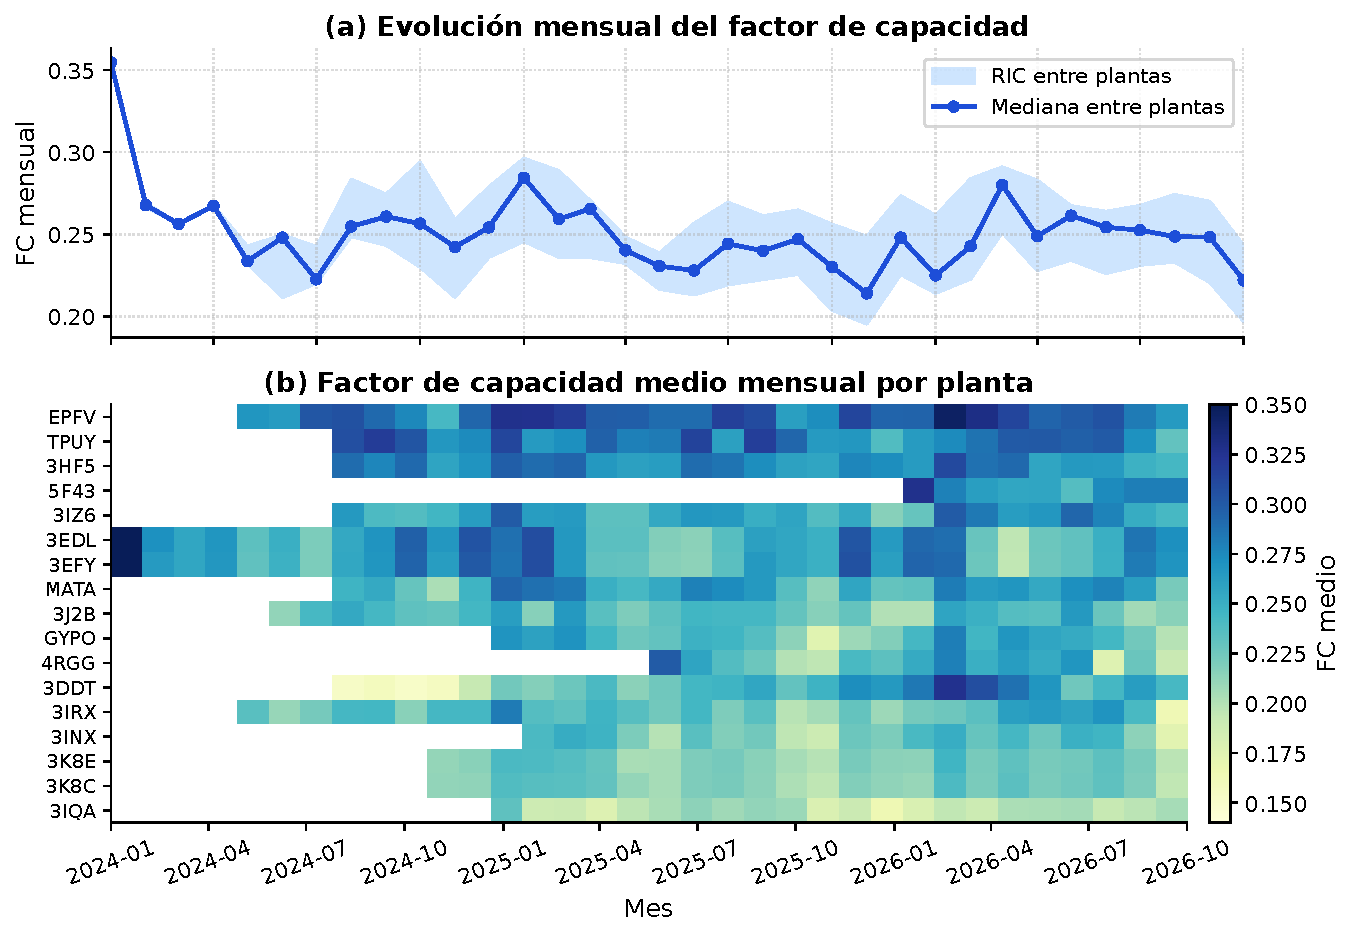
\includegraphics[width=0.92\textwidth]{figures/eda_estacionalidad.pdf}\\[0.5em]
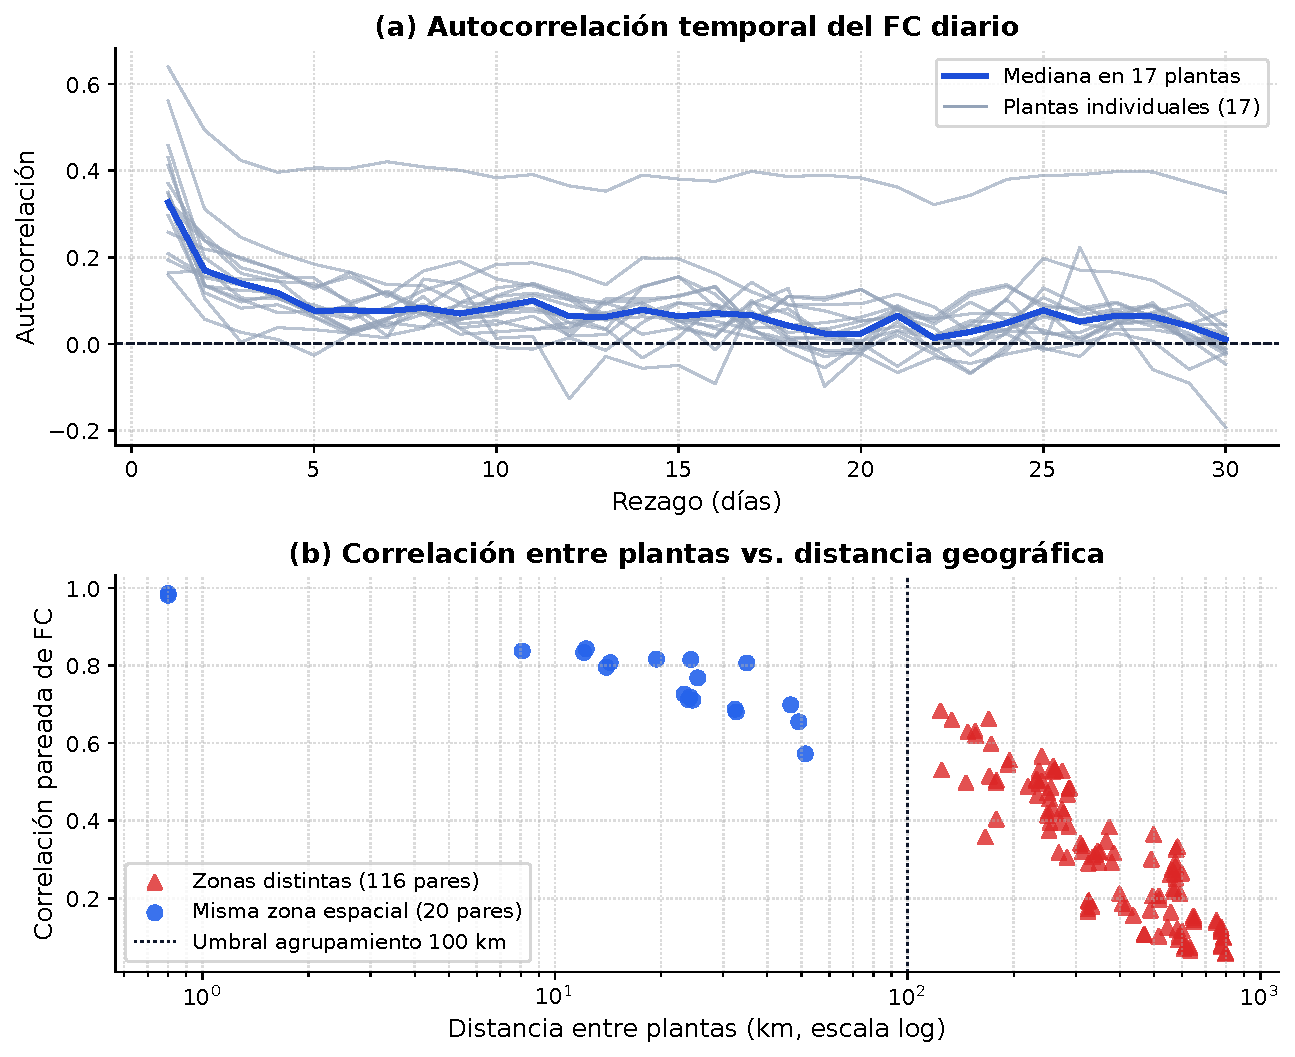
\includegraphics[width=0.92\textwidth]{figures/eda_dependencia.pdf}
\caption{Estacionalidad mensual del factor de capacidad (arriba) y estructura de autocorrelación temporal y correlación espacial entre centrales (abajo).}
\label{fig:eda_est_dep}
\end{figure}

\paragraph{4. ¿Qué comportamiento presentan las variables meteorológicas pronosticadas?}
Finalmente, la Figura~\ref{fig:eda_clima} muestra la distribución y dinámica de las cinco variables meteorológicas pronosticadas sobre la cohorte (irradiación horizontal, temperatura a $2\text{ m}$, nubosidad total, humedad relativa y velocidad del viento a $10\text{ m}$). La dispersión regional y la variabilidad atmosférica motivan complementar los niveles NWP absolutos con anomalías causales respecto a la media móvil reciente de $30$ días de cada planta y asignar una regularización cuadrática diferenciada ($\alpha_{\mathrm{meteo}}$) capaz de atenuar su influencia cuando la habilidad NWP se degrada en horizontes subestacionales.

\begin{figure}[!htbp]
\centering
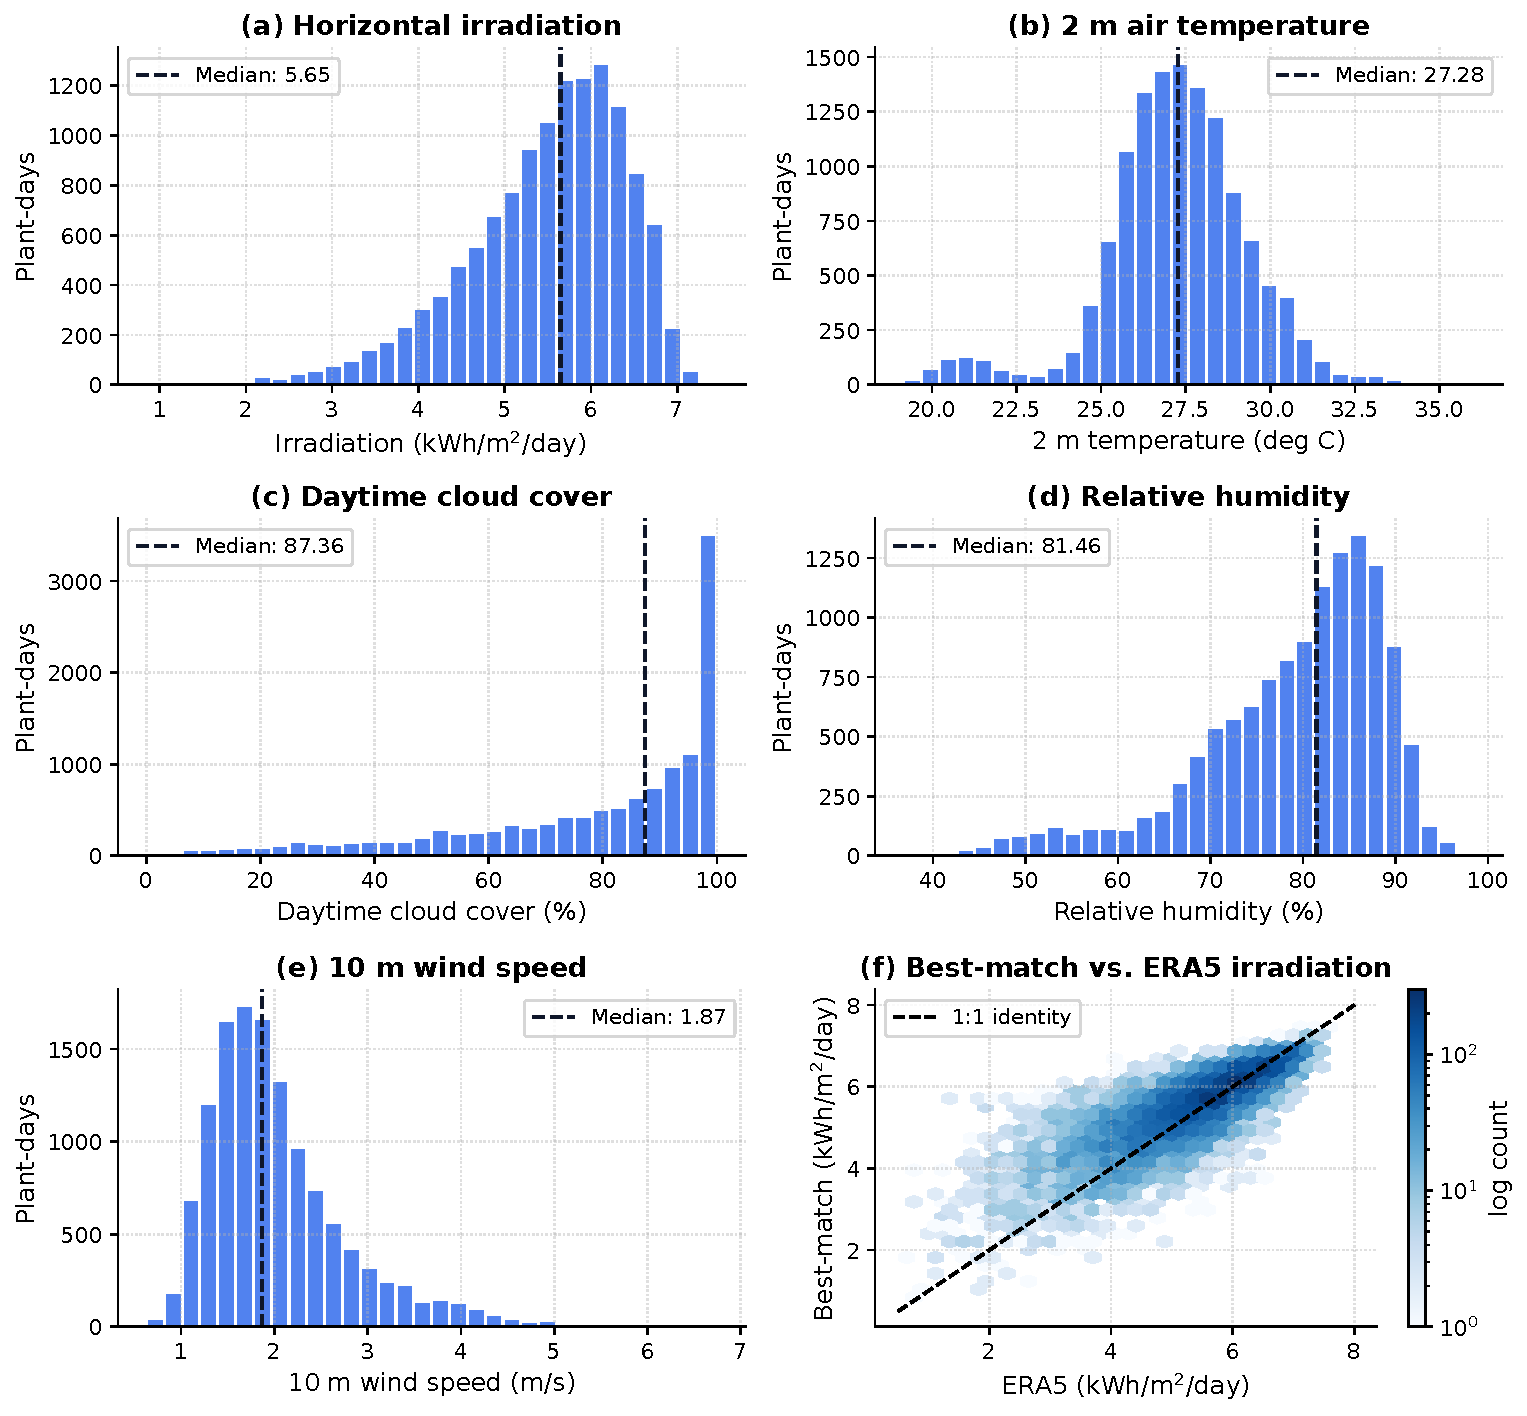
\includegraphics[width=0.92\textwidth]{figures/eda_clima.pdf}
\caption{Distribución y dinámica de las cinco variables meteorológicas pronosticadas sobre la cohorte de $17$ centrales.}
\label{fig:eda_clima}
\end{figure}

\section{Construcción matemática de los conjuntos experimentales}\label{sec:conjuntos}

Los $28$ escenarios evaluados corresponden a configuraciones experimentales derivadas sistemáticamente del mismo panel de $17$ centrales mediante combinaciones de horizonte, estrategia, disponibilidad meteorológica y régimen de generalización (Material Suplementario, Sección~S3, Tabla~S4), por lo que no constituyen $28$ conjuntos de datos independientes.

\subsection{Panel base, unidades físicas y filtración causal}

Sea $\mathcal{P} = \{1,\dots,M\}$ ($M=17$) el conjunto de centrales, cada una en una zona espacial fija $g(i) \in \{1,\dots,G\}$ ($G=7$), y sea $\mathcal{T}_i$ el conjunto de días válidos de la planta $i$ entre el 1 de enero de 2024 y el 31 de octubre de 2026. Con energía diaria $y_{i,s} > 0$ ($\text{kWh/día}$) y capacidad efectiva neta $C_{i,s} > 0$ ($\text{MW}$), la cota energética diaria bajo operación nominal continua de $24\text{ h}$ es:
\begin{equation}
E^{\max}_{i,s} := 24\,000\,C_{i,s} \quad (\text{kWh/día}).
\label{eq:emax}
\end{equation}
Al cierre operativo de un origen $t \in \mathcal{T}_i$, el denominador causal vigente es $E^{\max}_{i,t}$, evitando anticipar ampliaciones posteriores $C_{i,t+h}$ ($h \ge 1$). La filtración causal $\mathcal{F}_{i,t} := \sigma(\{y_{i,s}, C_{i,s} : s \le t\},\; \{\mathbf{z}_{i,u \mid s} : s \le t,\; u > s\},\; \text{calendario})$ agrupa observaciones pasadas y pronósticos emitidos en $s \le t$ para $u > s$. En todo el manuscrito, «causal» designa estrictamente no anticipación temporal respecto a $\mathcal{F}_{i,t}$.

\subsection{Definición de objetivos y representación de entrada}

Para planta $i$, origen $t$ y horizonte $H \in \{1,7,14,21,28\}$ días, se distinguen dos objetivos:
\begin{enumerate}
    \item \textbf{Objetivo diario ($D+1$ con $H=1$ y recursivo con $H \in \{7,14,21,28\}$):} para cada paso $h \in \{1,\dots,H\}$, la respuesta física es $y_{i,t+h}$ ($H_{\mathrm{dir}} = 1$) y su factor de capacidad causal truncado es:
    \begin{equation}
    c_{i,t+h \mid t} := \clip\!\left(\frac{y_{i,t+h}}{24\,000\,C_{i,t}},\, 0,\, 1\right),
    \qquad \clip(u,0,1) := \min\{\max\{u,0\},1\}.
    \label{eq:cf_diario}
    \end{equation}
    \item \textbf{Objetivo acumulado (esquema directo con $H \in \{7,14,21,28\}$):} predice en un paso la energía acumulada sobre ventanas válidas $[t+1, t+H]$ ($H_{\mathrm{dir}} = H$):
    \begin{equation}
    Y_{i,t}^{(H)} := \sum_{h=1}^{H} y_{i,t+h},
    \qquad
    c_{i,t}^{(H)} := \clip\!\left(\frac{Y_{i,t}^{(H)}}{24\,000\,H\,C_{i,t}},\, 0,\, 1\right),
    \label{eq:y_directo}
    \end{equation}
    dividiendo el error acumulado en $\text{kWh}$ por $H$ para expresarlo en $\text{kWh/día}$.
\end{enumerate}

A partir de las medias móviles causales de $30$ y $7$ días y del último registro válido hasta $t$ ($\bar{y}^{(30)}_{i,t}$, $\bar{y}^{(7)}_{i,t}$, $y^{\mathrm{ult}}_{i,t}$), se calculan los niveles recientes acotados:
\begin{equation}
\mathrm{cf}_{30}(i,t) := \clip\!\left(\frac{\bar{y}^{(30)}_{i,t}}{E^{\max}_{i,t}}, 0, 1\right),\quad
\mathrm{cf}_{7}(i,t) := \clip\!\left(\frac{\bar{y}^{(7)}_{i,t}}{E^{\max}_{i,t}}, 0, 1\right),\quad
\mathrm{cf}_{1}(i,t) := \clip\!\left(\frac{y^{\mathrm{ult}}_{i,t}}{E^{\max}_{i,t}}, 0, 1\right),
\label{eq:cf_hist}
\end{equation}
con respaldos jerárquicos causales en los primeros días sin ventana completa (Material Suplementario, Sección~S3). Para la fecha objetivo $t+h$, el vector de predictores $\mathbf{x}_{i,t+h \mid t} \in \mathbb{R}^p$ incluye:
\begin{itemize}
    \item \textbf{Sin meteorología ($p = 7$):} cuatro armónicos anuales evaluados en $t+h$ ($\sin/\cos$ de mes y día del año) y tres términos de dinámica autorregresiva con amortiguamiento geométrico $\gamma_h := 0{,}85^{h-1}$:
    \begin{equation}
    x_5 = \mathrm{cf}_{30}(i,t),\quad
    x_6 = \gamma_h \big(\mathrm{cf}_{7}(i,t) - \mathrm{cf}_{30}(i,t)\big),\quad
    x_7 = \gamma_h \big(\mathrm{cf}_{1}(i,t) - \mathrm{cf}_{7}(i,t)\big).
    \label{eq:features_din}
    \end{equation}
    \item \textbf{Con meteorología ($p = 17$):} añade las cinco variables pronosticadas $\mathbf{z}_{i,t+h \mid t}$ (irradiación horizontal, temperatura a $2\text{ m}$, nubosidad total, humedad relativa y viento a $10\text{ m}$) y cinco anomalías causales $\mathbf{a}_{i,t+h \mid t} = \mathbf{z}_{i,t+h \mid t} - \bar{\mathbf{z}}^{(30)}_{i,t}$ respecto a la media móvil de $30$ días de los pronósticos emitidos hasta $t$.
\end{itemize}

\subsection{Particiones externas, validación interna y actualización recursiva}

Las $28$ configuraciones cruzan cuatro familias de tarea ($D+1$ con y sin clima en tres bloques trimestrales nov-2025 a jul-2026; recursivo sin clima; directo acumulado sin clima; y recursivo con GEFSv12, con orígenes no solapados tras $90$ días de calentamiento para $H \in \{7,14,21,28\}$) con dos regímenes de generalización:
\begin{itemize}
    \item \textbf{Régimen intraplanta (IP):} al evaluar la fecha u origen $t_0$ de la planta $i$, $\mathcal{D}_{\mathrm{train}}(i,t_0)$ usa únicamente observaciones de la misma planta $i$ cuyo periodo objetivo concluye en $t_0$ o antes.
    \item \textbf{Régimen espaciotemporal (ET):} validación \textit{leave-one-group-out} sobre los $G=7$ conglomerados espaciales, entrenando con $\bigcup_{j : g(j) \ne g(i)} \mathcal{F}_{j,t_0}$. Este régimen \emph{no equivale a un escenario \textit{zero-shot} sin historial local}, pues la planta evaluada $i$ sí aporta su historial causal previo hasta $t_0$ ($\mathrm{cf}_{30}$, $\mathrm{cf}_7$, $\mathrm{cf}_1$ y $\bar{\mathbf{z}}^{(30)}_{i,t_0}$) para construir sus predictores al origen.
\end{itemize}

En \texttt{SM-CFHR-HPO}, la búsqueda interna ocurre dentro de $\mathcal{D}_{\mathrm{train}}$ mediante validación cruzada causal de $3$ particiones temporales (embargo de $30$ días en $D+1$; $t_{\mathrm{end}} \le t_{\mathrm{val}}$ en multihorizonte; exclusión espacial en ET). Para horizontes recursivos ($H \in \{7,14,21,28\}$), tanto la validación interna como la evaluación externa fijan $C_{i,t_0}$ y $\bar{\mathbf{z}}^{(30)}_{i,t_0}$ al origen e iteran paso a paso ($h=1,\dots,H$) desplazando el búfer histórico de $30$ días exclusivamente con las predicciones propias $\hat{y}_{i,t_0+h \mid t_0}$ (Material Suplementario, Sección~S3, Algoritmo~S1).

\section{Modelo SM-CFHR}\label{sec:modelo}

El estimador \textbf{SM-CFHR} (\textit{Structured Monotone Capacity-Factor Huber Regressor}) opera íntegramente en el espacio adimensional del factor de capacidad y reconstruye las predicciones en unidades de energía física al finalizar la inferencia. La Figura~\ref{fig:sm_cfhr_arq} sintetiza el flujo completo desde el panel de entrenamiento hasta la proyección física.

\begin{figure}[!htbp]
\centering
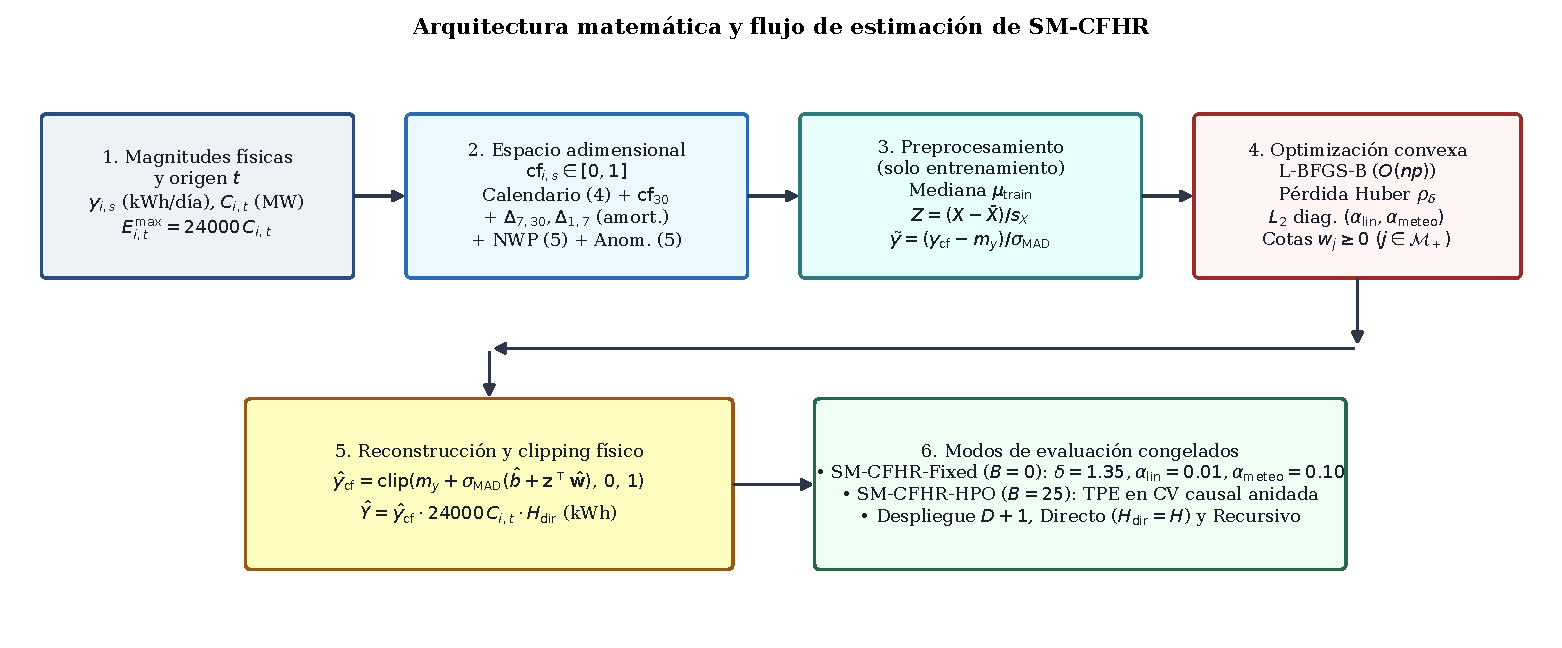
\includegraphics[width=0.98\textwidth]{figures/fig_sm_cfhr_arquitectura.pdf}
\caption{Arquitectura matemática de SM-CFHR: normalización causal por capacidad vigente, preprocesamiento sin fuga en entrenamiento, optimización convexa L-BFGS-B con pérdida de Huber y regularización $L_2$ diferenciada, y reconstrucción física acotada.}
\label{fig:sm_cfhr_arq}
\end{figure}

\subsection{Preprocesamiento en entrenamiento y escalado robusto MAD}

Sea $\mathcal{D}_{\mathrm{train}} = \{(\mathbf{x}_k, y_k)\}_{k=1}^n$ el conjunto de entrenamiento válido del pliegue (filtrando filas con $E^{\max}_k > 0$ y objetivo finito), con matriz de predictores $X \in \mathbb{R}^{n \times p}$ construida según la Sección~\ref{sec:conjuntos} ($p=7$ sin meteorología; $p=17$ con meteorología) y vector de factores de capacidad objetivo $\mathbf{y} \in [0,1]^n$ definido por \eqref{eq:cf_diario} o \eqref{eq:y_directo}. Todas las estadísticas de preprocesamiento se estiman exclusivamente sobre $\mathcal{D}_{\mathrm{train}}$:
\begin{enumerate}
    \item \textbf{Imputación por mediana:} cualquier valor no finito en la columna $j$ de $X$ se reemplaza por la mediana muestral $\mu_j = \mathrm{mediana}_k(X_{kj})$ calculada en $\mathcal{D}_{\mathrm{train}}$ (con respaldo $0$ si toda la columna es faltante), obteniendo $X^{\mathrm{imp}} \in \mathbb{R}^{n \times p}$.
    \item \textbf{Estandarización de predictores:} se calculan la media $\bar{x}_j = \frac{1}{n}\sum_{k=1}^n X^{\mathrm{imp}}_{kj}$ y la desviación estándar $s_j = \big(\frac{1}{n}\sum_{k=1}^n (X^{\mathrm{imp}}_{kj} - \bar{x}_j)^2\big)^{1/2}$. Para evitar inestabilidad numérica en columnas constantes, se define la escala efectiva $\tilde{s}_j = s_j$ si $s_j > 10^{-8}$ y $\tilde{s}_j = 1$ en caso contrario, produciendo la matriz estandarizada $Z \in \mathbb{R}^{n \times p}$ con entradas $Z_{kj} = (X^{\mathrm{imp}}_{kj} - \bar{x}_j)/\tilde{s}_j$.
    \item \textbf{Escalado robusto de la respuesta:} para que el umbral de transición $\delta > 0$ de la pérdida de Huber actúe en unidades adimensionales comparables entre centrales y estaciones, la respuesta se centra mediante la mediana $m_y = \mathrm{mediana}(\mathbf{y})$ y se escala mediante la desviación absoluta mediana $\mathrm{MAD}(\mathbf{y}) = \mathrm{mediana}(|\mathbf{y} - m_y|)$:
    \begin{equation}
    \sigma_y := \begin{cases}
    \max\{1{,}4826\,\mathrm{MAD}(\mathbf{y}),\; 10^{-6}\} & \text{si } \mathrm{MAD}(\mathbf{y}) > 0, \\
    \max\{\operatorname{std}(\mathbf{y}),\; 10^{-6}\} & \text{si } \mathrm{MAD}(\mathbf{y}) = 0,
    \end{cases}
    \qquad
    \tilde{y}_k := \frac{y_k - m_y}{\sigma_y}.
    \label{eq:mad_scale}
    \end{equation}
    La constante $1{,}4826 = 1/\Phi^{-1}(0{,}75)$ hace consistente a $\sigma_y$ con la desviación estándar bajo normalidad; el estimador MAD clásico posee punto de ruptura asintótico del $50\%$ \cite{rousseeuw1993mad}. En la implementación en NumPy (\texttt{\_robust\_target\_stats}), $m_y$ y $\mathrm{MAD}(\mathbf{y})$ se calculan mediante \texttt{np.median}, y cuando $\mathrm{MAD}(\mathbf{y}) = 0$ (cuando al menos la mitad de las observaciones coincide exactamente en $m_y$, contaminación por implosión) se activa el respaldo mediante la desviación estándar poblacional \texttt{np.std(..., ddof=0)} con piso numérico $10^{-6}$. Dado que la desviación estándar tiene punto de ruptura $0\%$ frente a valores atípicos, \emph{no} se demuestra ni se atribuye un punto de ruptura incondicional del $50\%$ al procedimiento compuesto por tramos \eqref{eq:mad_scale}.
\end{enumerate}

\subsection{Función objetivo, regularización estructurada y restricciones de signo}

Denotemos por $\mathbf{z}_k \in \mathbb{R}^p$ la $k$-ésima fila de $Z$. SM-CFHR estima un intercepto no penalizado $b \in \mathbb{R}$ y un vector de coeficientes $\mathbf{w} \in \mathbb{R}^p$ resolviendo el programa convexo:
\begin{equation}
\min_{b \in \mathbb{R},\; \mathbf{w} \in \mathcal{C}} \; J(b, \mathbf{w}) := \frac{1}{n}\sum_{k=1}^{n} \rho_\delta\!\left(\tilde{y}_k - b - \mathbf{z}_k^\top \mathbf{w}\right) + \frac{1}{2}\mathbf{w}^\top D_\alpha \mathbf{w},
\label{eq:objetivo_smcfhr}
\end{equation}
donde $\rho_\delta : \mathbb{R} \to \mathbb{R}_{\ge 0}$ es la pérdida de Huber con umbral $\delta > 0$,
\begin{equation}
\rho_\delta(r) := \begin{cases}
\frac{1}{2} r^2 & \text{si } |r| \le \delta, \\
\delta\left(|r| - \frac{1}{2}\delta\right) & \text{si } |r| > \delta,
\end{cases}
\label{eq:huber}
\end{equation}
la matriz diagonal $D_\alpha = \diag(d_1,\dots,d_p)$ asigna penalizaciones cuadráticas diferenciadas por familia de predictores,
\begin{equation}
d_j := \begin{cases}
\alpha_{\mathrm{meteo}} & \text{si } j \in \mathcal{G}_{\mathrm{meteo}}, \\
\alpha_{\mathrm{lin}} & \text{si } j \notin \mathcal{G}_{\mathrm{meteo}},
\end{cases}
\label{eq:d_alpha}
\end{equation}
siendo $\mathcal{G}_{\mathrm{meteo}} = \{8,\dots,17\}$ el bloque de variables meteorológicas y anomalías ($\mathcal{G}_{\mathrm{meteo}} = \emptyset$ cuando no hay meteorología), y el conjunto factible $\mathcal{C} \subseteq \mathbb{R}^p$ impone restricciones de no negatividad sobre el subconjunto de índices físicamente monótonos $\mathcal{M}_+$:
\begin{equation}
\mathcal{C} := \{\mathbf{w} \in \mathbb{R}^p : w_j \ge 0 \;\forall j \in \mathcal{M}_+\},
\quad
\mathcal{M}_+ = \begin{cases}
\{5, 8\} \text{ ($\mathrm{cf}_{30}$ e irradiación pronosticada)} & \text{con clima}, \\
\{5\} \text{ ($\mathrm{cf}_{30}$)} & \text{sin clima}.
\end{cases}
\label{eq:conjunto_factible}
\end{equation}

Desde el punto de vista estadístico, \eqref{eq:objetivo_smcfhr} extiende la regresión Ridge \cite{hoerl1970} y los híbridos robustos analizados por Owen~\cite{owen2007} en dos direcciones específicas del problema fotovoltaico. Por un lado, $D_\alpha$ permite aplicar una contracción moderada ($\alpha_{\mathrm{lin}}$) sobre la dinámica autorregresiva y el calendario, mientras regula con mayor intensidad ($\alpha_{\mathrm{meteo}}$) las variables NWP para mitigar el sobreajuste ante la degradación meteorológica de mediano plazo. Por otro lado, las cotas $w_j \ge 0$ para $j \in \mathcal{M}_+$ impiden que la colinealidad entre predictores produzca pendientes negativas físicamente espurias respecto al nivel base reciente o a la irradiación pronosticada.

El modelo se evalúa bajo dos presupuestos experimentales bien delimitados:
\begin{itemize}
    \item \textbf{SM-CFHR-Fixed ($B=0$):} configuración congelada con $\delta = 1{,}35$, $\alpha_{\mathrm{lin}} = 0{,}01$ y $\alpha_{\mathrm{meteo}} = 0{,}10$ (en ausencia de meteorología, $d_j = \alpha_{\mathrm{lin}}$ para todo $j$), sin búsqueda interna de hiperparámetros.
    \item \textbf{SM-CFHR-HPO ($B=25$):} optimización bayesiana TPE mediante Optuna dentro de cada pliegue externo sobre el espacio continuo $\delta \in [0{,}5, 3{,}0]$, $\alpha_{\mathrm{lin}} \in [10^{-4}, 1{,}0]$ (escala logarítmica) y, cuando hay meteorología, $\alpha_{\mathrm{meteo}} \in [10^{-3}, 10{,}0]$ (escala logarítmica). En los escenarios recursivos, la validación interna evalúa cada candidato mediante el mismo Algoritmo~\ref{alg:rollout} de despliegue causal exacto.
\end{itemize}

\subsection{Reconstrucción física y modos de despliegue}

Para un vector de consulta $\mathbf{x}_q \in \mathbb{R}^p$, se aplica la imputación $\mu_j$ y la estandarización $\mathbf{z}_q = (\mathbf{x}^{\mathrm{imp}}_q - \bar{\mathbf{x}})/\tilde{\mathbf{s}}$ con los parámetros del entrenamiento. A partir de la solución óptima $(\hat{b}, \hat{\mathbf{w}})$, el factor de capacidad y la energía física predichos se obtienen mediante:
\begin{equation}
\widehat{\mathrm{cf}}_q := \clip\!\left(m_y + \sigma_y \big(\hat{b} + \mathbf{z}_q^\top \hat{\mathbf{w}}\big),\; 0,\; 1\right),
\qquad
\hat{y}_q := \widehat{\mathrm{cf}}_q \cdot 24\,000\,C_{i,t} \cdot H_{\mathrm{dir}} \quad (\text{kWh}),
\label{eq:pred_fisica}
\end{equation}
con respaldo al promedio histórico $\bar{y}^{(30)}_{i,t}\,H_{\mathrm{dir}}$ si $C_{i,t}$ no fuese finita, acotado al intervalo físico $[0, 24\,000\,H_{\mathrm{dir}}\,C_{i,t}]$.

La Figura~\ref{fig:despliegue_mh} contrasta los tres modos de despliegue: (1) $D+1$ ($H=1$, $H_{\mathrm{dir}}=1$), que evalúa \eqref{eq:pred_fisica} una sola vez; (2) el esquema directo acumulado ($H \in \{7,14,21,28\}$, $H_{\mathrm{dir}}=H$), que entrena y predice directamente sobre la energía total de la ventana $[t+1, t+H]$ sin realimentación; y (3) el esquema recursivo multihorizonte ($H \in \{7,14,21,28\}$, $H_{\mathrm{dir}}=1$), que entrena en $h=1$ e itera el Algoritmo~\ref{alg:rollout} realimentando exclusivamente sus propias predicciones. Conviene subrayar que, aunque el ajuste interno \eqref{eq:objetivo_smcfhr} es un programa convexo, la composición recursiva de $H$ pasos realimentando $\hat{y}_{i,t_0+h \mid t_0}$ es una función no lineal y no convexa de los parámetros.

\begin{figure}[!htbp]
\centering
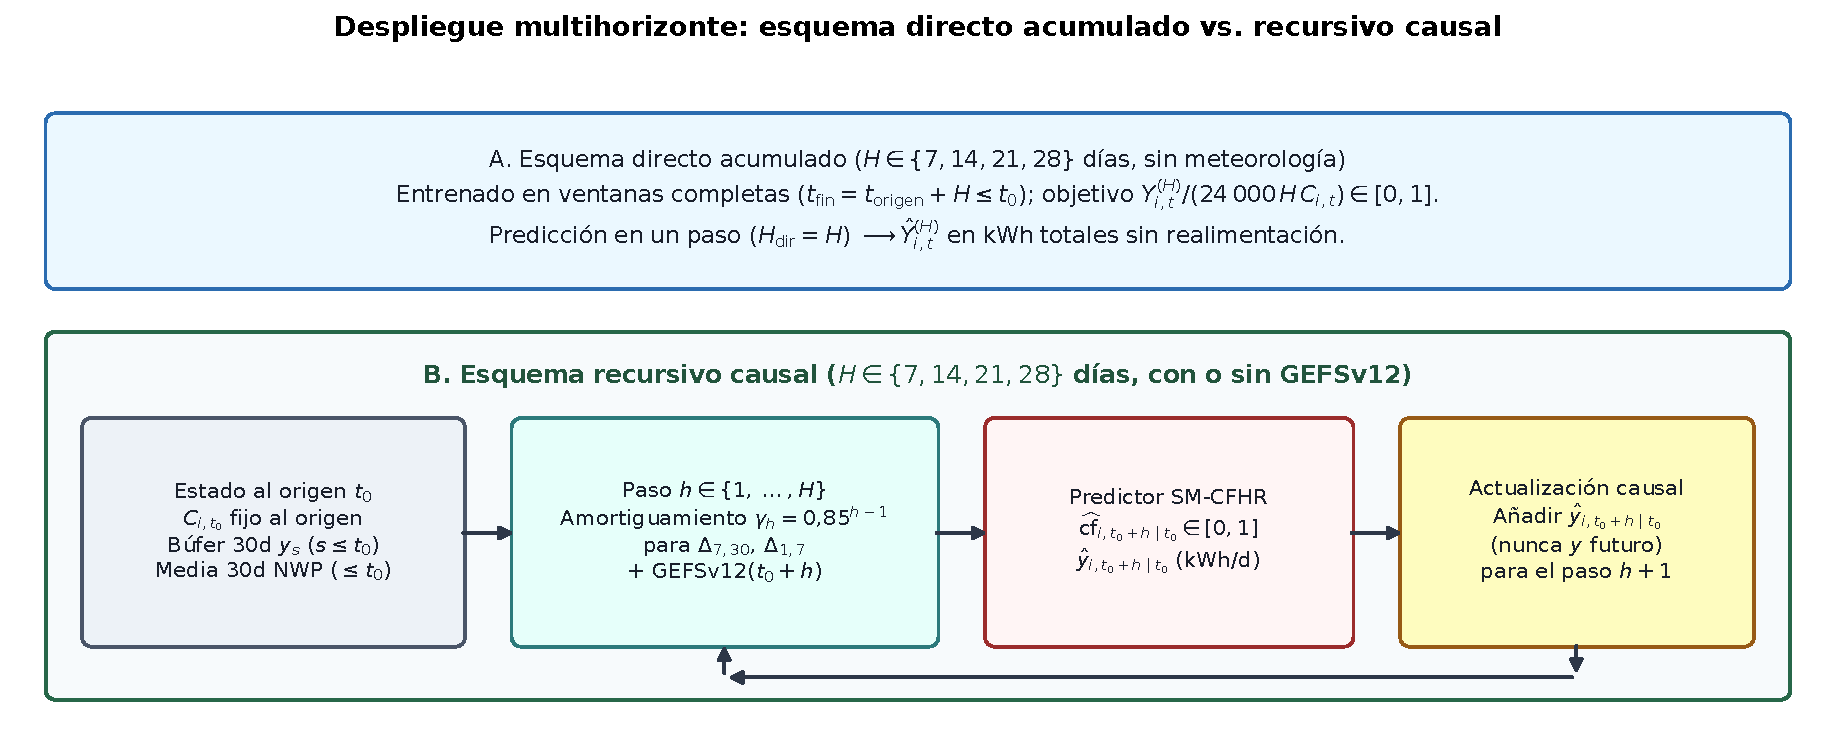
\includegraphics[width=0.98\textwidth]{figures/fig_despliegue_multihorizonte.pdf}
\caption{Comparación estructural entre el esquema directo acumulado ($H_{\mathrm{dir}}=H$, sin realimentación) y el despliegue recursivo multihorizonte con actualización causal mediante predicciones propias y amortiguamiento geométrico.}
\label{fig:despliegue_mh}
\end{figure}

\section{Propiedades matemáticas y verificación formal}\label{sec:propiedades}

El programa \eqref{eq:objetivo_smcfhr} admite una caracterización analítica completa en regularidad diferencial, convexidad, existencia, unicidad, condiciones de optimalidad y sensibilidad (demostraciones completas, matriz Hessiana por tramos y análisis de complejidad en el Material Suplementario, Sección~S1 y Figura~S6).

\subsection{Gradiente analítico y regularidad $C^1$}

La derivada de Huber $\psi_\delta(r) := \rho_\delta'(r) = \clip(r, -\delta, \delta)$ es continua y $1$-Lipschitz en $\mathbb{R}$. Definiendo el vector de residuos $\mathbf{r}(b, \mathbf{w}) := \tilde{\mathbf{y}} - b\mathbf{1}_n - Z\mathbf{w} \in \mathbb{R}^n$, el gradiente exacto de $J$ es:
\begin{equation}
\frac{\partial J}{\partial b}(b,\mathbf{w}) = -\frac{1}{n}\sum_{k=1}^{n} \psi_\delta(r_k), \qquad
\nabla_{\mathbf{w}} J(b,\mathbf{w}) = -\frac{1}{n} Z^\top \psi_\delta(\mathbf{r}) + D_\alpha \mathbf{w}.
\label{eq:gradiente_smcfhr}
\end{equation}
La función objetivo $J$ es de clase $C^1(\mathbb{R}^{p+1})$ con gradiente Lipschitz continuo, pero no es $C^2$ sobre los hiperplanos $|r_k(b,\mathbf{w})| = \delta$, donde la segunda derivada presenta saltos finitos. Esta regularidad $C^1$ por tramos justifica el uso de L-BFGS-B \cite{byrd1995lbfgsb,zhu1997lbfgsb}: emplea únicamente evaluaciones de $J$, gradientes analíticos de primer orden y proyecciones simples sobre $\mathbb{R} \times \mathcal{C}$ con coste $O(np)$ por evaluación, evitando invertir Hessianas discontinuas.

\subsection{Convexidad, existencia, unicidad, KKT e influencia}

Distinguiendo las consecuencias directas de la teoría convexa \cite{boyd2004convex} y estimación $M$ \cite{huber1964,huber2009robust} frente a las propiedades específicas de un intercepto no penalizado bajo pérdida de Huber:

\begin{theorem}[Convexidad y existencia de soluciones]\label{thm:convexidad_existencia}
Si $n \ge 1$, $\delta > 0$, $\alpha_{\mathrm{lin}} > 0$ y $\alpha_{\mathrm{meteo}} > 0$, entonces: (1) $\Omega := \mathbb{R} \times \mathcal{C}$ es cerrado y convexo en $\mathbb{R}^{p+1}$; (2) $J \in C^1(\mathbb{R}^{p+1})$ es convexa con gradiente globalmente Lipschitz de constante $L_J \le \frac{1}{n}\left\|\begin{bmatrix}\mathbf{1}_n & Z\end{bmatrix}\right\|_2^2 + \max\{\alpha_{\mathrm{lin}}, \alpha_{\mathrm{meteo}}\}$; y (3) $J$ es coerciva sobre $\Omega$ y acotada inferiormente por $0$, garantizando al menos un minimizador global $(b^*, \mathbf{w}^*) \in \Omega$.
\end{theorem}

\begin{theorem}[Unicidad exacta y caso degenerado del intercepto]\label{thm:unicidad}
Bajo las hipótesis del Teorema~\ref{thm:convexidad_existencia}: (1) el vector óptimo de coeficientes $\mathbf{w}^* \in \mathcal{C}$ es \textbf{único}; (2) si existe al menos una observación $k$ con $|\tilde{y}_k - b^* - \mathbf{z}_k^\top \mathbf{w}^*| < \delta$ para algún $b^*$ óptimo, entonces el intercepto $b^*$ también es \textbf{único}; y (3) si $|r_k(b^*,\mathbf{w}^*)| \ge \delta$ para todo $k$ (con $n$ par e igual número de residuos positivos y negativos), el conjunto de interceptos óptimos puede ser un intervalo no degenerado.
\end{theorem}

Dado que $\mathcal{C}$ está definido por desigualdades afines y satisface la condición de Slater ($w_j = 1 > 0$ para $j \in \mathcal{M}_+$), las condiciones KKT son necesarias y suficientes para la optimalidad global (Material Suplementario, Sección~S1, Proposición~S1): en particular, cuando una cota $w_j^* = 0$ ($j \in \mathcal{M}_+$) está activa, la correlación residual ponderada cumple $\frac{1}{n}(Z^\top \psi_\delta(\mathbf{r}^*))_j \le 0$. Asimismo, aunque $|\psi_\delta(r_k)| \le \delta$ acota la influencia de cada observación en la respuesta ($\delta/n$ en el intercepto y $(\delta/n)\|\mathbf{z}_k\|_\infty$ en los pesos), SM-CFHR \emph{no} posee función de influencia acotada frente a puntos de apalancamiento arbitrarios en covariables $\|\mathbf{z}_k\|$ \cite{hampel1986robust}. Por último, para todo $j \in \mathcal{M}_+$ con $\tilde{s}_j > 0$, $\hat{y}_q$ es monótona no decreciente en $x_{q,j}$ \textit{ceteris paribus} y permanece en $[0, 24\,000\,H_{\mathrm{dir}}\,C_{i,t}]$, sin garantizar monotonía conjunta si múltiples covariables correlacionadas varían simultáneamente.

\subsection{Verificación formal en Lean~4}\label{sec:lean4_resumen}

Los resultados analíticos anteriores fueron formalizados en \textbf{Lean~4} (\texttt{leanprover/lean4:v4.36.0}) \cite{moura2021lean4} sobre \textbf{Mathlib} \cite{mathlib2020} (Material Suplementario, Sección~S2, Tabla~S1), compilando $26$ declaraciones verificadas en seis módulos sobre $\mathbb{R}$ sin axiomas personalizados (únicamente \texttt{propext}, \texttt{Classical.choice} y \texttt{Quot.sound}). La formalización distingue hipótesis explícitas ($n \ge 1$ y $\alpha_j > 0$ para coercividad/existencia frente a $\alpha_j \ge 0$ para convexidad/KKT) y demuestra la regularidad Lipschitz de $\partial J/\partial b$ (\texttt{gradB\_lipschitz}), mientras la cota espectral completa $L_J$ de $\nabla J$ se demuestra analíticamente en la Sección~S1. La verificación en $\mathbb{R}$ no cubre aritmética IEEE-754 ni convergencia numérica de L-BFGS-B.

\section{Protocolo de evaluación e inferencia estadística}\label{sec:inferencia}

La evaluación experimental se organiza en dos etapas metodológicas explícitamente separadas para preservar la trazabilidad de las predicciones primarias: (1) la evaluación fuera de muestra (OOF) primaria sobre $28$ configuraciones frente a $22$ referencias en energía bruta, y (2) la reconciliación de estimandos inferenciales y métricas adimensionales sobre esas mismas predicciones guardadas, junto con los estudios diagnósticos en $D+1$. En ningún caso se alteran ni regeneran las predicciones OOF primarias.

\subsection{Métricas, validación anidada y transparencia de presupuestos}

Para evaluar el desempeño en una flota con coberturas heterogéneas ($251$ a $1\,032$ días útiles) y capacidades entre $9{,}8$ y $388{,}0$~MW, el protocolo congelado emplea como métrica primaria el \textbf{error absoluto medio macro por planta}:
\begin{equation}
\mathrm{MAE}_{\mathrm{macro}}(m) := \frac{1}{M}\sum_{i=1}^{M}\frac{1}{|\mathcal{T}_i^{\mathrm{eval}}|}\sum_{t \in \mathcal{T}_i^{\mathrm{eval}}} e_{m,i,t},
\label{eq:mae_macro}
\end{equation}
donde $e_{m,i,t} = |y_{i,t+1} - \hat{y}_{i,t+1 \mid t}|$ en $D+1$ ($\text{kWh/día}$), $e_{m,i,t} = \frac{1}{H}\sum_{h=1}^{H}|y_{i,t+h} - \hat{y}_{i,t+h \mid t}|$ en esquema recursivo ($\text{kWh/día}$) y $e_{m,i,t} = |Y_{i,t}^{(H)} - \hat{Y}_{i,t}^{(H)}|$ en esquema directo ($\text{kWh}$ totales, reportando además su equivalente normalizado por $H$ en $\text{kWh/día}$). Conviene precisar tres aspectos de escala y nomenclatura: (i) promediar primero por planta iguala la ponderación respecto a la duración de las series ($|\mathcal{T}_i^{\mathrm{eval}}|$), pero al expresarse en $\text{kWh/día}$ los errores absolutos siguen siendo proporcionales a la capacidad instalada de cada central ($9{,}8$ frente a $388{,}0$~MW); (ii) seis centrales de la cohorte (\texttt{3HF5}, \texttt{3IZ6}, \texttt{EPFV}, \texttt{GYPO}, \texttt{MATA}, \texttt{TPUY}) registran ampliaciones escalonadas de capacidad entre $2024$ y $2026$, por lo que el MAE adimensional en factor de capacidad $\mathrm{MAE}_{\mathrm{CF,macro}}$ divide cada error por $24\,000\,C_{i,t}$ (y por $H$ en directos) usando la capacidad vigente al origen; y (iii) la razón relativa respecto a la generación media observada por planta se etiqueta explícitamente como $\mathrm{nMAE}_{\mathrm{rel,gen}}$ para no confundirla con $\mathrm{MAE}_{\mathrm{CF,macro}}$, mientras que $\mathrm{Skill}_{\mathrm{RMSE}}$ se define exclusivamente frente a \texttt{MM30}.

Para controlar el sesgo de selección \cite{varma2006bias,cawley2010overfit} y transparentar las diferencias de presupuesto de búsqueda entre variantes, distinguimos dos niveles de comparación sobre las $28$ configuraciones experimentales (Figura~\ref{fig:validacion_anidada}):
\begin{itemize}
    \item \textbf{Comparación primaria (\texttt{SM-CFHR-Fixed}, $B=0$):} evalúa la configuración fija ($\delta = 1{,}35$, $\alpha_{\mathrm{lin}} = 0{,}01$, $\alpha_{\mathrm{meteo}} = 0{,}10$) sin optimización de hiperparámetros frente a los $22$ modelos de referencia (los cuales emplearon una rejilla acotada de $4$ configuraciones).
    \item \textbf{Comparación secundaria (\texttt{SM-CFHR-HPO}, $B=25$):} evalúa la variante optimizada mediante $25$ ensayos Optuna TPE dentro de cada pliegue externo sobre $3$ particiones causales internas (embargo de $30$ días en $D+1$, $t_{\mathrm{end}} \le t_{\mathrm{val}}$ en multihorizonte, y exclusión espacial estricta en ET). Reportar por separado $B=0$ y $B=25$ evita atribuir a la arquitectura del modelo ganancias que pudieran provenir de un mayor presupuesto de búsqueda.
\end{itemize}

\begin{figure}[!htbp]
\centering
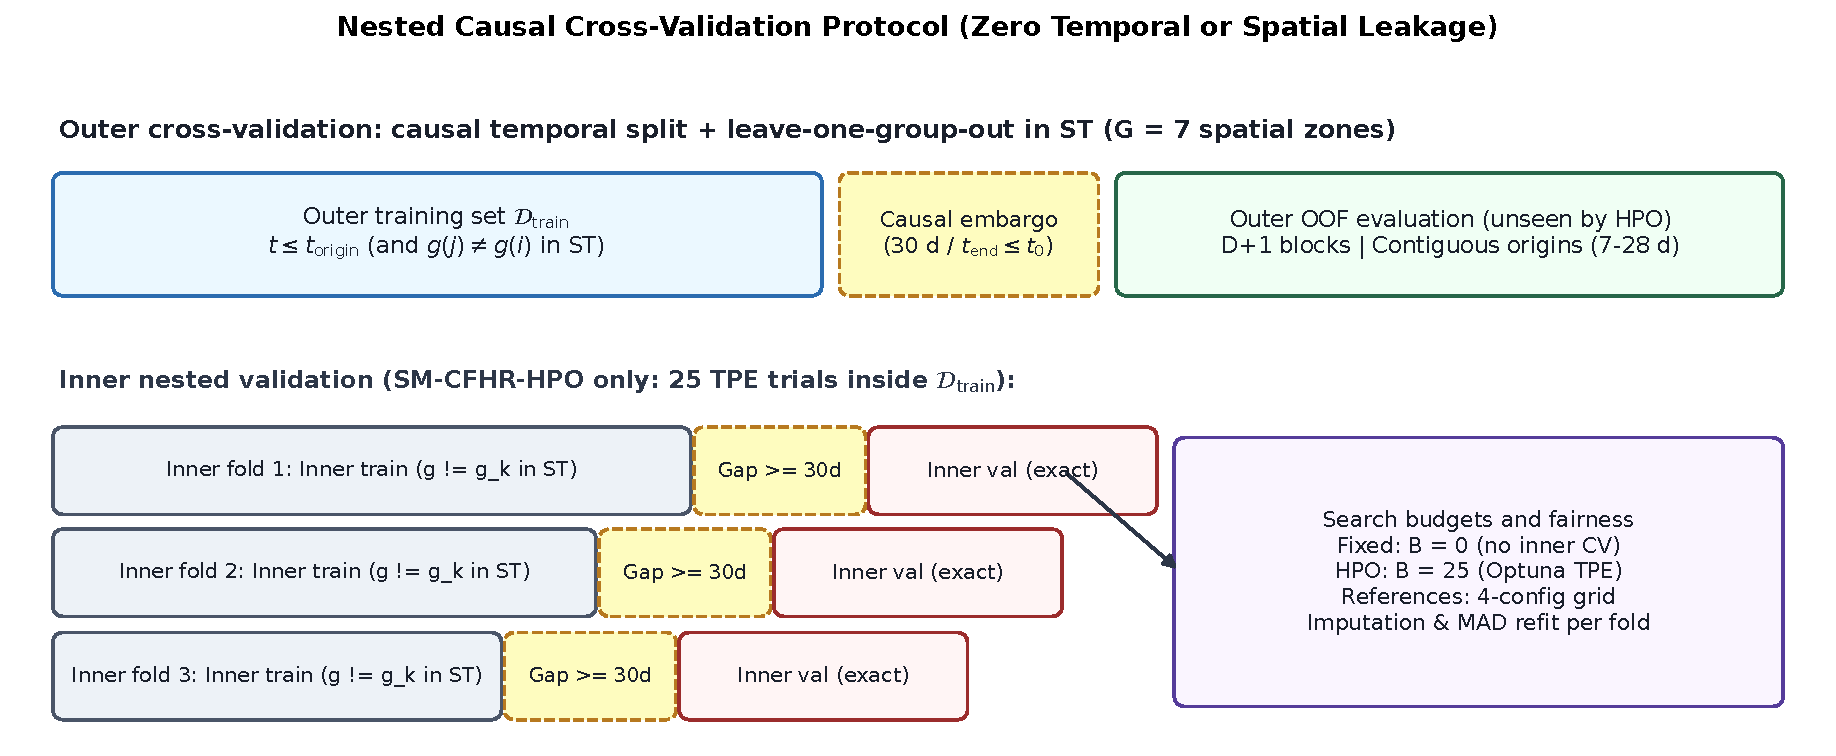
\includegraphics[width=0.98\textwidth]{figures/fig_validacion_anidada.pdf}
\caption{Esquema de validación cruzada causal anidada: separación temporal y espacial externa (\textit{leave-one-group-out} en ET) con brecha de embargo causal de $30$ días y validación interna de $3$ particiones para Optuna TPE.}
\label{fig:validacion_anidada}
\end{figure}

\subsection{Contrastes pareados, multiplicidad y calibración ante autocorrelación}

Para comparar dos procedimientos $m_A$ y $m_B$ sobre series temporales alineadas (agregadas por fecha en $D+1$ y por origen en multihorizonte), definimos el diferencial de pérdida $d_t := L_{m_A, t} - L_{m_B, t}$ para $t = 1,\dots,T$ (valores negativos favorecen a $m_A$). Ante la autocorrelación serial propia de series diarias y de horizontes solapados $H$, la varianza de largo plazo se estima mediante el estimador HAC de Newey--West \cite{newey1987} con núcleo de Bartlett hasta el rezago $L = \max\{1, \lfloor 4(T/100)^{2/9} \rfloor\}$:
\begin{equation}
\hat{\Omega}_{\mathrm{HAC}} := \hat{\gamma}_0 + 2\sum_{k=1}^{L}\left(1 - \frac{k}{L+1}\right)\hat{\gamma}_k, \qquad
\hat{\gamma}_k := \frac{1}{T}\sum_{t=k+1}^{T}(d_t - \bar{d})(d_{t-k} - \bar{d}),
\label{eq:hac}
\end{equation}
y el tamaño muestral efectivo se cuantifica como
\begin{equation}
T_{\mathrm{eff}} := \frac{T}{\max\!\left\{1,\; 1 + 2\sum_{k=1}^{L}\left(1 - \frac{k}{L+1}\right)\frac{\hat{\gamma}_k}{\hat{\gamma}_0}\right\}}.
\end{equation}
Cuando $T_{\mathrm{eff}} < 2H$ (frecuente en horizontes $H \in \{21, 28\}$ días con orígenes no solapados), el protocolo inicial declaraba el escenario con tamaño muestral efectivo insuficiente. La reconciliación inferencial posterior identificó dos desajustes en esa formulación: (a) en los escenarios multihorizonte, los orígenes consecutivos están separados exactamente por $H$ días, por lo que no existe solapamiento entre ventanas ($h_{\mathrm{serie}} = 1$, no $H$); y (b) el promedio simple por origen no coincide con $\mathrm{MAE}_{\mathrm{macro}}$ cuando varía el número de plantas disponibles por origen ($1$ a $17$). Para mantener trazabilidad completa sin alterar las predicciones primarias, la reconciliación añade la serie temporal macro-alineada $z_t^{\mathrm{macro}} = \frac{T}{M}\sum_{i \in \mathcal{P}_t} S_{t,i}/N_i$ (cuya media temporal coincide idénticamente con $\Delta\mathrm{MAE}_{\mathrm{macro}}$), bootstrap estacionario sincronizado entre plantas, política explícita para series de varianza nula ($\Delta=0 \Rightarrow p=1{,}0$; $\Delta \neq 0$ constante $\Rightarrow p=\text{NaN}$, no evaluable por DM asintótico), niveles de fiabilidad muestral según $T_{\mathrm{eff}}$ ($<2h_{\mathrm{serie}}$, $[2h_{\mathrm{serie}},20)$, $[20,30)$, $\ge 30$) y la verificación de SPA/MCS con $B=5\,000$ réplicas (Material Suplementario, Sección~S4).

Sobre los escenarios que superan $T_{\mathrm{eff}} \ge 2H$, se distinguen los procedimientos integrados en la evaluación primaria frente a los análisis complementarios post-hoc:
\begin{enumerate}
    \item \textbf{Diebold--Mariano con corrección HLN y varianza HAC:} estadístico bilateral frente a $t_{T-1}$ bajo $H_0 : \mathbb{E}[d_t] = 0$ \cite{diebold1995,harvey1997,newey1987}. La comparación preespecificada frente a una referencia única corresponde a la línea base causal \texttt{MM30} (y al contraste pareado entre \texttt{SM-CFHR-Fixed} y \texttt{SM-CFHR-HPO}). En cambio, el contraste frente a la «mejor referencia de biblioteca» seleccionada \textit{ex post} sobre la misma muestra de evaluación está sujeto a sesgo de selección posterior que vuelve anticonservadora la calibración nominal; asimismo, las comparaciones frente a representantes individuales de biblioteca (\texttt{Ridge}, \texttt{XGBoost}) tienen carácter exploratorio.
    \item \textbf{Model Confidence Set (MCS):} eliminación secuencial al nivel $\alpha = 0{,}10$ con estadístico $T_{\max}$ sobre los $23$ modelos simultáneos \cite{hansen2011mcs,politis1994stationary} ($B=200$ réplicas en el protocolo inicial y $B=5\,000$ en la reconciliación macro-alineada, con longitud media de bloque $7$). Permanecer en el MCS indica que no existe evidencia al nivel $\alpha = 0{,}10$ para descartar al modelo como inferior respecto al conjunto superviviente, pero no implica automáticamente significancia pareada frente a cada modelo excluido.
    \item \textbf{Prueba global SPA (análisis post-hoc):} contraste de capacidad predictiva superior con recentrado consistente, $B=500$ a $5\,000$ réplicas de bootstrap estacionario y longitud media de bloque $7$ \cite{hansen2005spa}. Cuando una referencia actúa como $H_0$, rechazarla ($p_{\mathrm{SPA}} < 0{,}05$) indica que al menos un competidor la supera; cuando SM-CFHR actúa como $H_0$, no rechazarla no demuestra superioridad ni equivalencia.
    \item \textbf{Giacomini--White (GW) y Clark--West (CW):} GW \cite{giacomini2006tests} se excluye como prueba confirmatoria cuando $\tau=1$ y $|\hat{\rho}_1| > 0{,}15$ tras verificar sobrerrechazo bajo errores $\mathrm{AR}(1)$ ($0{,}2083$ frente a $0{,}05$ nominal en $120$ simulaciones exploratorias); CW \cite{clark2007nested} se reserva estrictamente para modelos anidados.
\end{enumerate}

Para controlar las comparaciones múltiples dentro de cada familia de escenarios, se aplican la corrección secuencial de Holm--Bonferroni \cite{holm1979} (control de FWER) y el ajuste de Benjamini--Hochberg \cite{benjamini1995fdr} (control de FDR) únicamente sobre los escenarios con $T_{\mathrm{eff}} \ge 2H$. La magnitud práctica de las diferencias se cuantifica mediante $\bar{d}$ con intervalo de confianza al $95\%$ por bootstrap estacionario ($1\,000$ réplicas), la $d$ de Cohen pareada y el delta de Cliff no paramétrico \cite{cliff1993dominance}, manteniendo cautela inferencial por tratarse de $G=7$ conglomerados espaciales \cite{cameron2015cluster}.

\subsection{Hipótesis científicas preespecificadas y estudios diagnósticos}

El protocolo contrasta cuatro hipótesis científicas una vez concluidas las evaluaciones fuera de muestra:
\begin{itemize}
    \item \textbf{H1 (Ventaja de normalización en transferencia espacial):} en generalización espaciotemporal (ET), la normalización causal por factor de capacidad reduce el $\mathrm{MAE}_{\mathrm{macro}}$ frente a regresores globales entrenados sin normalización de escala.
    \item \textbf{H2 (Significancia pareada y relevancia práctica bajo dependencia temporal):}
    \begin{enumerate}
        \item \textit{Hipótesis científica principal:} en los escenarios con tamaño muestral efectivo $T_{\mathrm{eff}} \ge 2H$, SM-CFHR reduce el error fuera de muestra respecto a la referencia preespecificada \texttt{MM30} (y, de forma exploratoria, frente a la mejor referencia de biblioteca y rivales representativos).
        \item \textit{Contrastes pareados y corrección múltiple:} se evalúa mediante la prueba DM--HLN--HAC bilateral ajustada por Holm--Bonferroni ($p_{\mathrm{Holm}} < 0{,}05$) y Benjamini--Hochberg dentro de cada familia de escenarios.
        \item \textit{Tamaños del efecto y relevancia práctica:} se reportan como criterios descriptivos complementarios la $d$ de Cohen pareada ($|d_{\mathrm{Cohen}}| \ge 0{,}20$), el delta de Cliff ($|\delta_{\mathrm{Cliff}}| \ge 0{,}147$) y el intervalo al $95\%$ por bootstrap estacionario.
        \item \textit{Procedimientos complementarios de conjunto:} la pertenencia al MCS ($\alpha=0{,}10$, integrado en el flujo OOF) y la prueba SPA (post-hoc) aportan contexto de conjunto, sin combinar todas las pruebas en un único test ni interpretar la supervivencia en MCS o el no rechazo de SPA como demostración de superioridad pareada.
    \end{enumerate}
    \item \textbf{H3 (Contribución de componentes estructurales):} la pérdida de Huber ($\delta=1{,}35$), la regularización anisotrópica ($\alpha_{\mathrm{meteo}} > \alpha_{\mathrm{lin}}$) y las restricciones de monotonía no negativa aportan mejoras verificables o mayor estabilidad ante atípicos respecto a sus versiones ablacionadas.
    \item \textbf{H4 (Compromiso entre configuración fija y HPO):} la optimización bayesiana TPE ($B=25$) mejora o iguala a la configuración fija congelada ($B=0$) en regímenes con señal meteorológica suficiente sin incurrir en sobreajuste por varianza de selección.
\end{itemize}

Para investigar la contribución de cada componente constructivo (H3) y caracterizar el comportamiento del estimador sobre el panel real $D+1$ con corte cronológico estricto ($\max t_{\mathrm{train}} < \min t_{\mathrm{val}}$), se ejecutan los siguientes estudios diagnósticos:
\begin{enumerate}
    \item \textbf{Ablación controlada en $D+1$ ($6$ variantes):} contrasta \texttt{SM-CFHR\_completo} frente a cinco modificaciones sobre el mismo panel y corte: (a) $\delta = 10^6$ para aproximar pérdida cuadrática $L_2$ (\texttt{sin\_huber\_L2}); (b) regularización isotrópica $\alpha_{\mathrm{meteo}} = \alpha_{\mathrm{lin}}$ (\texttt{sin\_l2\_estructurada}); (c) supresión de cotas $w_j \ge 0$ (\texttt{sin\_monotonia}); (d) estandarización externa manteniendo MAD (\texttt{escala\_std\_vs\_mad}); y (e) ajuste directo en energía bruta $\text{kWh/día}$ (\texttt{energia\_bruta\_vs\_cf}).
    \item \textbf{Sensibilidad, semillas y estrés sintético en $D+1$:} barridos unidimensionales sobre $(\delta, \alpha_{\mathrm{lin}}, \alpha_{\mathrm{meteo}})$, estabilidad en $10$ semillas ($2026$--$2035$) y estrés ante contaminación en entrenamiento ($0\%$, $5\%$ y $10\%$ de perturbaciones $\pm 0{,}6$ en factor de capacidad con ruido gaussiano $\sigma=0{,}10$ en predictores).
    \item \textbf{Incertidumbre conforme temporal e interpretabilidad aditiva:} intervalos conformes divididos al $80\%$ y $90\%$ nominales mediante cuantiles de residuos absolutos pasados \cite{vovk2005conformal,lei2018conformal,barber2023nonexchangeable}, e importancia aditiva exacta $\phi_{q,j} = \sigma_y (z_{q,j} - \bar{z}_{\mathrm{train},j})\,\hat{w}_j$.
\end{enumerate}

\subsection{Coste computacional y reproducibilidad}

Sobre las $28$ configuraciones ($14\,625$ unidades por variante, $206\,073$ filas de predicción), \texttt{SM-CFHR-Fixed} ($B=0$) concluyó en $499{,}75$~s ($8{,}33$~min) con $8$ trabajadores, frente a $29\,550{,}3$~s ($8{,}21$~h) de \texttt{SM-CFHR-HPO} ($B=25$) con $12$ trabajadores ($59\times$ mayor tiempo de pared). Las especificaciones completas de hardware, entorno Python, semilla global~$2026$ y tolerancia a fallos figuran en el Material Suplementario (Sección~S4).

\section{Resultados}\label{sec:resultados}

Los resultados se presentan siguiendo las dos etapas del estudio sobre las predicciones OOF primarias ($28$ configuraciones, $14\,625$ unidades por variante, cero errores): el desempeño frente a las $22$ referencias oficiales en energía bruta, y su reconciliación inferencial y en factor de capacidad adimensional, junto con los estudios diagnósticos en $D+1$.

\subsection{Desempeño global en las 28 configuraciones y comparación Fixed vs.\ HPO}

Sobre el soporte común alineado con los $22$ modelos de referencia en energía bruta ($\text{kWh}$), \texttt{SM-CFHR-Fixed} ($B=0$) alcanza un rango ordinal medio de $\mathbf{2{,}93/23}$ en $\mathrm{MAE}_{\mathrm{macro}}$ ($\text{kWh}$), obtiene $\mathbf{18/28}$ victorias descriptivas frente al mejor competidor de biblioteca (\texttt{Mejor\_Bib}, $10/28$ derrotas), $\mathbf{22/28}$ frente al mejor modelo residual (\textit{custom}) y $\mathbf{15/28}$ frente a \texttt{MM30} (Tabla~\ref{tab:res_familias}). Por régimen y familia, el desempeño es marcadamente asimétrico:
\begin{itemize}
    \item \textbf{Horizonte $D+1$ y generalización espaciotemporal (ET):} en $D+1$ ET con cinco variables logra rango $1/23$ con reducción de $-22{,}16\%$ frente a \texttt{Mejor\_Bib} ($59\,803{,}6$ frente a $76\,831{,}1$~kWh/día, $\mathrm{Skill}=28{,}80\%$ sobre \texttt{MM30}). En $D+1$ intraplanta con clima obtiene $61\,297{,}1$~kWh/día (rango $12/23$, $-0{,}22\%$ frente a biblioteca).
    \item \textbf{Esquema recursivo sin clima ($7$--$28$~días):} mantiene rango medio $2{,}00/23$ en ET ($4/4$ victorias sobre biblioteca, $-1{,}70\%$ medio) y $1{,}50/23$ en intraplanta ($3/4$ victorias sobre biblioteca, $-0{,}27\%$ medio), aunque por debajo de \texttt{MM30} en ET.
    \item \textbf{Esquema directo acumulado sin clima ($7$--$28$~días):} es competitivo en ET ($3/4$ victorias frente a biblioteca, rango medio $3{,}25/23$, $-1{,}63\%$ medio), pero se degrada sistemáticamente en intraplanta ($1/4$ victorias, $+13{,}27\%$ medio, alcanzando $+24{,}24\%$ en $H=28$~días frente a \texttt{k-NN}).
    \item \textbf{Acoplamiento con NOAA GEFSv12 ($7$--$28$~días):} en ET alcanza rango $\mathbf{1{,}00/23}$ en los cuatro horizontes ($4/4$ victorias frente a biblioteca y \texttt{MM30}, $-11{,}84\%$ medio frente a biblioteca); en intraplanta obtiene rango medio $2{,}00/23$ ($0/4$ frente a biblioteca, $+1{,}04\%$, pero $4/4$ sobre \texttt{MM30}).
\end{itemize}

\begin{table}[!htbp]
\caption{Resumen comparativo por familia de escenarios de \texttt{SM-CFHR-Fixed} ($B=0$) sobre el soporte común alineado ($28$ escenarios, $23$ modelos en $\text{kWh}$).}\label{tab:res_familias}
\centering
\scriptsize
\begin{tabular}{llccccc}
\toprule
Familia & Tarea & Esc. & Rango medio & Vic.\ vs.\ Bib. & Vic.\ vs.\ MM30 & $\Delta$ medio vs.\ Bib. (\%) \\
\midrule
$D+1$ & Espaciotemporal & $2$ & $1{,}00$ & $2/2$ & $2/2$ & $-11{,}30\%$ \\
$D+1$ & Intraplanta & $2$ & $7{,}50$ & $1/2$ & $2/2$ & $+0{,}07\%$ \\
Directo sin clima & Espaciotemporal & $4$ & $3{,}25$ & $3/4$ & $0/4$ & $-1{,}63\%$ \\
Directo sin clima & Intraplanta & $4$ & $6{,}50$ & $1/4$ & $0/4$ & $+13{,}27\%$ \\
Rec.\ sin clima & Espaciotemporal & $4$ & $2{,}00$ & $4/4$ & $0/4$ & $-1{,}70\%$ \\
Rec.\ sin clima & Intraplanta & $4$ & $1{,}50$ & $3/4$ & $3/4$ & $-0{,}27\%$ \\
Rec.\ + GEFSv12 & Espaciotemporal & $4$ & $1{,}00$ & $4/4$ & $4/4$ & $-11{,}84\%$ \\
Rec.\ + GEFSv12 & Intraplanta & $4$ & $2{,}00$ & $0/4$ & $4/4$ & $+1{,}04\%$ \\
\bottomrule
\end{tabular}
\end{table}

Al comparar directamente ambas variantes mediante $\mathrm{MAE}_{\mathrm{macro}}$, \texttt{SM-CFHR-HPO} ($B=25$, $14\,552$ estudios Optuna con $25$ ensayos válidos y $73$ unidades sin historial suficiente) solo mejora a \texttt{SM-CFHR-Fixed} ($B=0$) en $\mathbf{9/28}$ escenarios ---todos intraplanta---, mientras \texttt{Fixed} vence en $14/14$ escenarios espaciotemporales y $5/14$ intraplanta ($19/28$ en total; rango medio $2{,}93$ frente a $3{,}86/23$), con un coste de pared $59\times$ menor (Figura~\ref{fig:res_oof_rankings}).

\begin{figure}[!htbp]
\centering
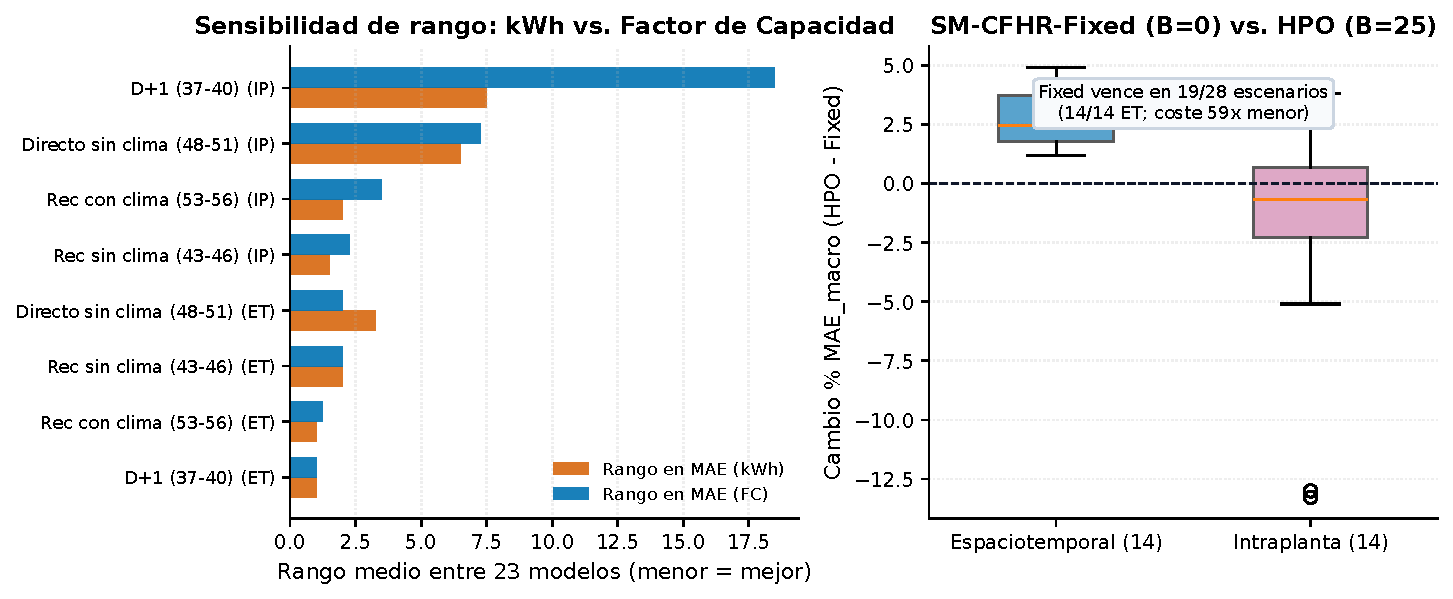
\includegraphics[width=0.98\textwidth]{figures/fig_res_oof_rankings_y_fixed_hpo.pdf}
\caption{Evaluación OOF primaria y métricas adimensionales: sensibilidad del rango medio entre $\text{kWh}$ ($2{,}93/23$) y factor de capacidad ($4{,}00/23$), y comparación pareada entre \texttt{SM-CFHR-Fixed} ($B=0$) y \texttt{SM-CFHR-HPO} ($B=25$).}
\label{fig:res_oof_rankings}
\end{figure}

\subsection{Protocolo original (v1.0.3), análisis retrospectivo (v2.0.0) y métricas en factor de capacidad}

Bajo el protocolo original congelado \texttt{v1.0.3} ($T_{\mathrm{eff}} \ge 2H$ sobre promedios simples por origen), únicamente $2/15$ contrastes DM--HLN--HAC frente a \texttt{Mejor\_Bib} alcanzaban significancia tras Holm ($D+1$ ET con clima y \texttt{RecGEFSv12} ET $7$d), excluyendo $13$ escenarios de horizontes largos. En la adaptación inferencial retrospectiva \texttt{v2.0.0} sobre los $28$ escenarios completos a partir de las mismas predicciones OOF guardadas sin reentrenar:
\begin{enumerate}
    \item \textbf{Inversiones de signo entre $\mathrm{MAE}_{\mathrm{macro}}$ y promedio por origen:} el desbalance de disponibilidad entre plantas ($1$ a $17$ centrales por origen) invertía el signo de $\Delta\mathrm{MAE}$ en $4/28$ escenarios (\texttt{D1\_IP\_sin\_clima}, \texttt{RecSinClima\_IP\_14d}, \texttt{RecSinClima\_IP\_28d} y \texttt{DirectoSinClima\_IP\_7d}), ninguno significativo ($p \ge 0{,}28$).
    \item \textbf{DM--HLN--HAC y bootstrap sincronizado sobre $\mathrm{MAE}_{\mathrm{macro}}$ (análisis retrospectivo):} con $h_{\mathrm{serie}}=1$ en bloques disjuntos y serie macro-alineada $z_t^{\mathrm{macro}}$, todos los $5/5$ escenarios \texttt{ET + Clima} ($D+1$ y $7$, $14$, $21$, $28$~días) muestran diferencias estadísticamente significativas tras Holm por familia frente a \texttt{Mejor\_Bib} seleccionado \textit{ex post} ($p_{\mathrm{Holm}} \le 5{,}21\times 10^{-6}$), manteniendo $0$ diferencias significativas en régimen intraplanta o sin clima. Debe destacarse como cautela muestral que en \texttt{RecGEFSv12 ET} de $21$ y $28$ días los tamaños efectivos se sitúan cerca del umbral descriptivo de $30$ ($T_{\mathrm{eff,macro}} = 31{,}35$ y $30{,}82$, respectivamente) con solo $G=7$ zonas espaciales. Frente a referencias preespecificadas en el diseño, \texttt{SM-CFHR-Fixed} obtiene $7/28$ diferencias favorables significativas ($0$ desfavorables) frente a \texttt{MM30} y $4/28$ frente a \texttt{SM-CFHR-HPO} ($1/28$ desfavorable).
    \item \textbf{Análisis secundario retrospectivo frente a las $9$ bibliotecas ($252$ contrastes):} en el archivo de reconciliación \texttt{v2.0.0} sobre el universo global de $252$ comparaciones ($9$ bibliotecas $\times$ $28$ escenarios), todas las $45/45$ comparaciones pareadas en los cinco escenarios \texttt{ET + Clima} presentan diferencia macro favorable ($\Delta\mathrm{MAE}_{\mathrm{macro}} < 0$) y resultan significativas bajo Holm global ($p_{\mathrm{Holm,252}} < 0{,}05$, con máximos por escenario de $9{,}03\times 10^{-22}$ en $D+1$, $1{,}41\times 10^{-9}$ en $7$d, $1{,}34\times 10^{-5}$ en $14$d, $3{,}58\times 10^{-3}$ en $21$d y $4{,}17\times 10^{-2}$ en $28$d). Este resultado proviene de un análisis exploratorio retrospectivo sobre la cohorte ya estudiada y no constituye una validación prospectiva independiente.
    \item \textbf{SPA y MCS ($B=5\,000$):} en \texttt{MCS} ($T_{\max}$ unilateral) sobre $\mathrm{MAE}_{\mathrm{macro}}$, \texttt{SM-CFHR-Fixed} sobrevive en $27/28$ escenarios del universo completo y como único superviviente ($1/10$) en $7/28$ entre bibliotecas (Material Suplementario, Sección~S4).
    \item \textbf{Métricas reales en factor de capacidad ($\mathrm{MAE}_{\mathrm{CF,macro}}$):} al normalizar cada observación por $24\,000\,C_{i,t}$ vigente (incluidas las $6$ centrales con ampliaciones escalonadas), el peso de las plantas mayores (como \texttt{GYPO}, $370$--$388$~MW) deja de dominar la media. El rango medio de \texttt{SM-CFHR-Fixed} pasa de $2{,}93/23$ ($\text{kWh}$) a $\mathbf{4{,}00/23}$ (CF), y las victorias descriptivas frente a \texttt{Mejor\_Bib} de $18/28$ a $16/28$.
\end{enumerate}

Las Figuras~\ref{fig:res_oof_planta}, \ref{fig:res_oof_d1}, \ref{fig:res_oof_rec} y \ref{fig:res_oof_dir} ilustran el desempeño por planta y grupo espacial (con capacidad diaria causal al origen y soporte pareado) junto con trayectorias ilustrativas en $D+1$, recursivo multihorizonte y directo acumulado.

\begin{figure}[!htbp]
\centering
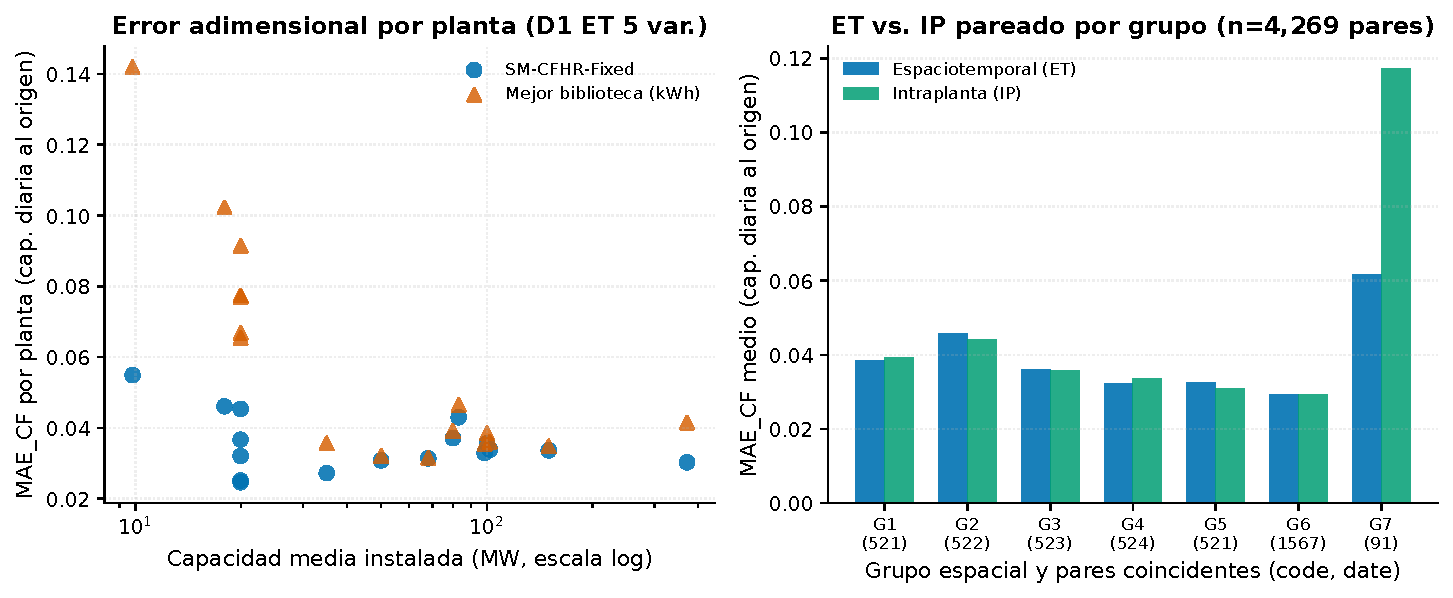
\includegraphics[width=0.98\textwidth]{figures/fig_res_oof_planta_y_grupos.pdf}
\caption{Error adimensional $\mathrm{MAE}_{\mathrm{CF}}$ por planta (normalizado observación por observación con la capacidad diaria al origen) frente a la capacidad media en \texttt{D1\_ET\_5var} (izquierda) y comparación ET frente a IP estrictamente pareada por \texttt{(code, date)} en los $7$ grupos espaciales ($n=4\,269$ pares coincidentes; grupo~7 con $n=91$ pares frente a $134$ en ET sin parear; derecha).}
\label{fig:res_oof_planta}
\end{figure}

\begin{figure}[!htbp]
\centering
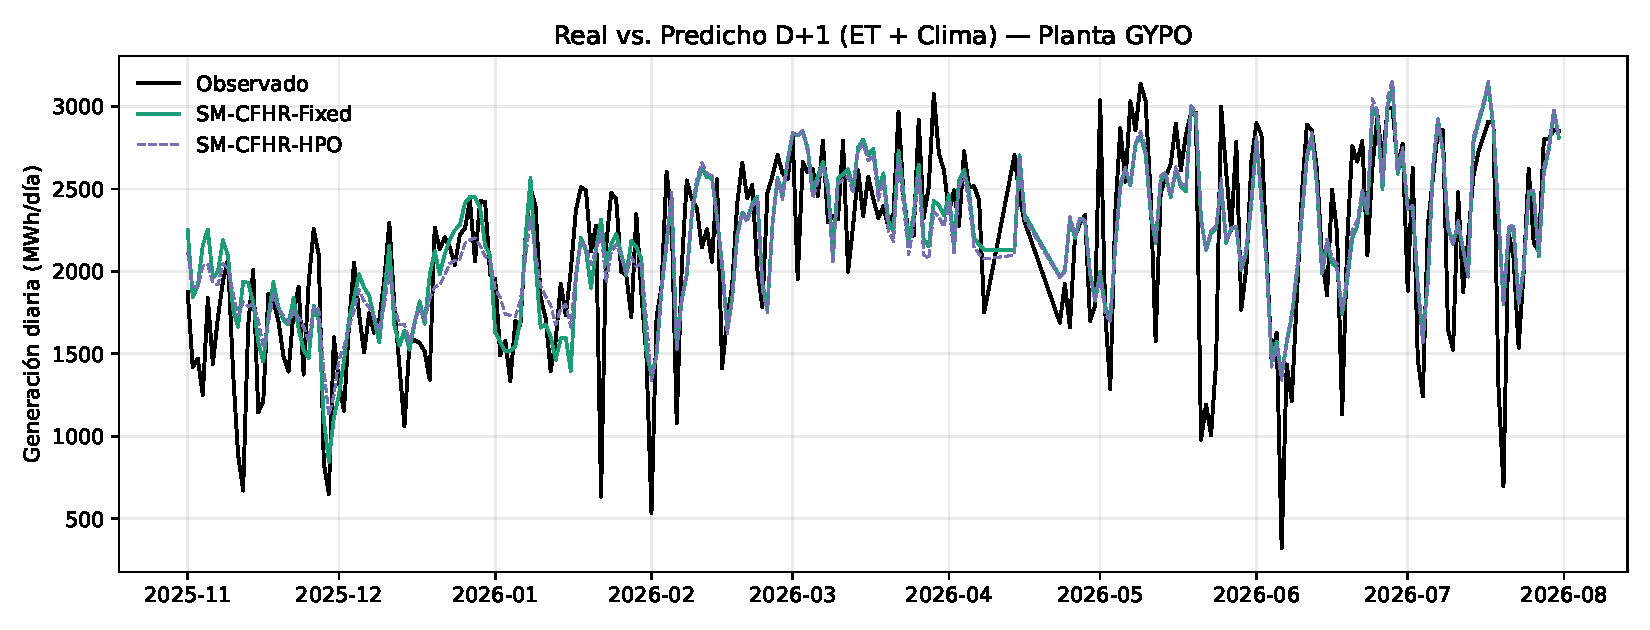
\includegraphics[width=0.95\textwidth]{figures/fig_res_oof_real_vs_pred_d1.pdf}
\caption{Ejemplo ilustrativo de generación diaria real frente a predicha en $D+1$ (\texttt{D1\_ET\_5var}, noviembre de $2025$ a julio de $2026$) para la central \texttt{GYPO}, seleccionada por registrar la mayor generación media y capacidad instalada de la cohorte ($370$--$388$~MW).}
\label{fig:res_oof_d1}
\end{figure}

\begin{figure}[!htbp]
\centering
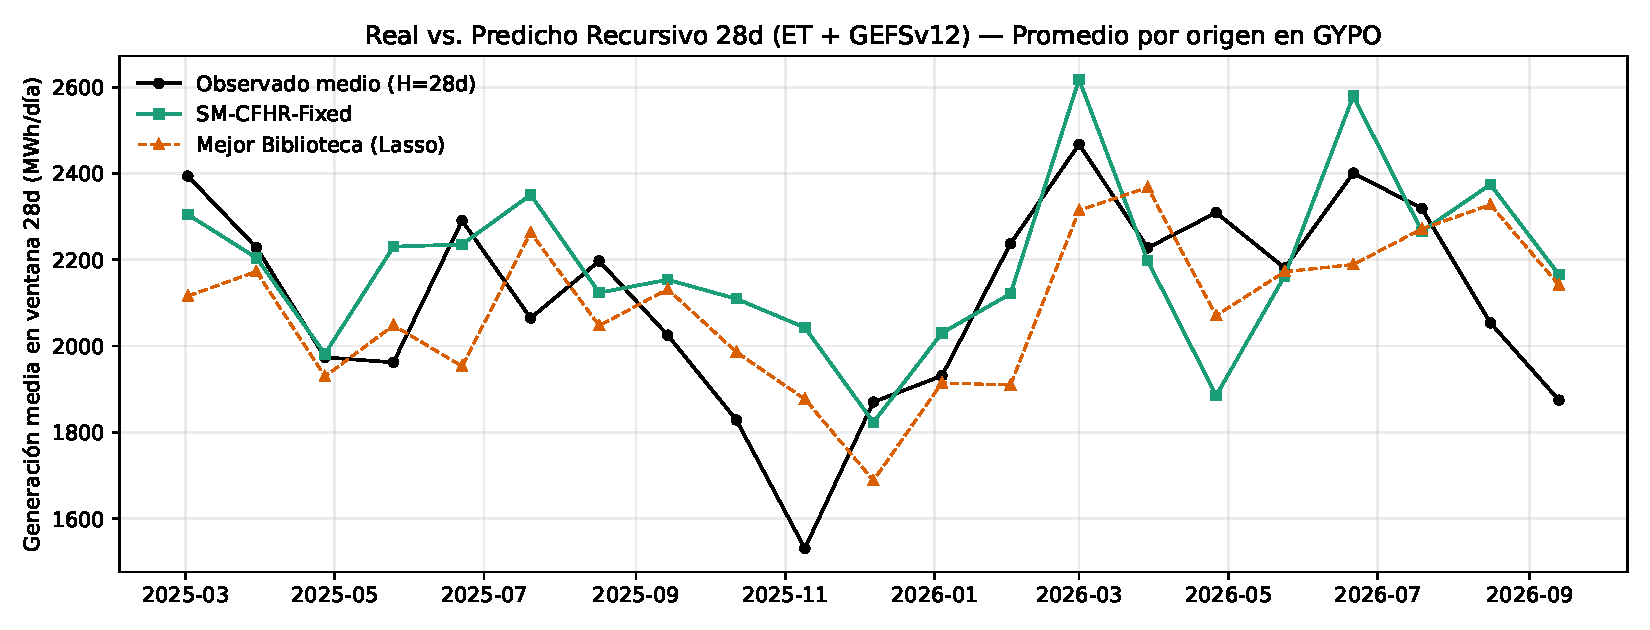
\includegraphics[width=0.95\textwidth]{figures/fig_res_oof_real_vs_pred_rec.pdf}
\caption{Ejemplo ilustrativo de trayectorias promedio por origen ($H=28$~días) reales frente a predichas en el esquema recursivo con meteorología GEFSv12 (\texttt{RecGEFSv12\_ET\_28d}, marzo de $2025$ a septiembre de $2026$) para la central \texttt{GYPO} (mayor generación media de la cohorte).}
\label{fig:res_oof_rec}
\end{figure}

\begin{figure}[!htbp]
\centering
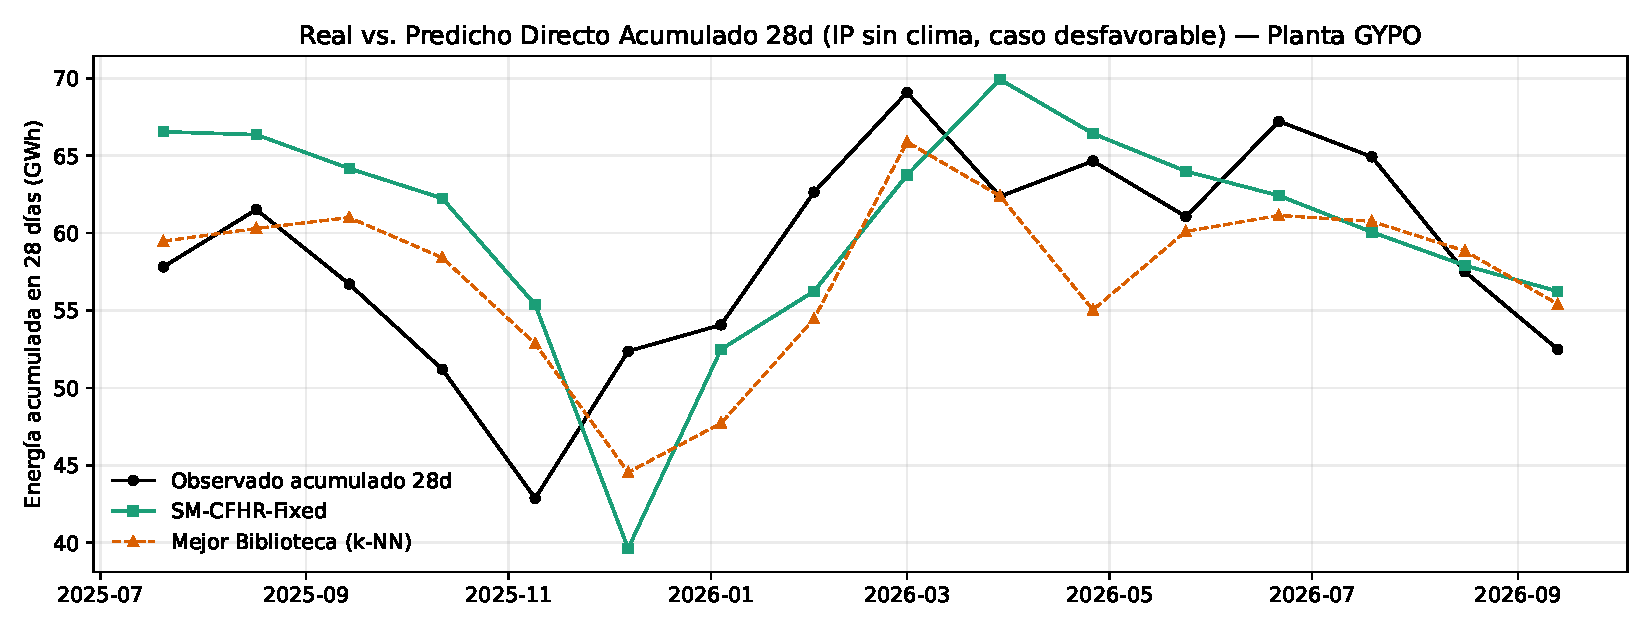
\includegraphics[width=0.95\textwidth]{figures/fig_res_oof_real_vs_pred_dir.pdf}
\caption{Ejemplo ilustrativo de energía acumulada en ventanas de $28$~días observada frente a predicha en el esquema directo sin meteorología (\texttt{DirectoSinClima\_IP\_28d}, caso desfavorable) para la central \texttt{GYPO} (seleccionada por mayor generación media de la cohorte, no como muestra aleatoria).}
\label{fig:res_oof_dir}
\end{figure}

\subsection{Estudios diagnósticos en $D+1$: ablación, estrés, incertidumbre e interpretabilidad}

Sobre el panel real $D+1$ con corte cronológico estricto ($\max t_{\mathrm{train}} < \min t_{\mathrm{val}}$) se observan los siguientes resultados (Tabla~\ref{tab:res_ablaciones} y Figura~\ref{fig:res_oof_ablaciones}):
\begin{enumerate}
    \item \textbf{Ablación controlada en $D+1$:} suprimir la normalización por factor de capacidad (\texttt{energia\_bruta\_vs\_cf}) multiplica el error por $4{,}45\times$ ($270\,035{,}5$ frente a $60\,631{,}2$~kWh/día; $0{,}23065$ frente a $0{,}03488$ CF). La pérdida de Huber mejora marginalmente sobre $L_2$ en datos limpios ($60\,631{,}2$ frente a $60\,784{,}0$~kWh/día), mientras \texttt{sin\_monotonia} y \texttt{escala\_std\_vs\_mad} coinciden con el modelo completo en este corte porque los pesos naturales de \texttt{cf30} ($+0{,}4591$) y \texttt{rad\_pron} ($+0{,}0863$) ya resultaron positivos.
    \item \textbf{Semillas y estrés sintético en $D+1$:} \texttt{SM-CFHR-Fixed} es determinista en las $10$ semillas ($56\,437{,}8$~kWh/día constantes), frente a la variabilidad de \texttt{HPO} ($55\,660{,}9$--$59\,124{,}8$~kWh/día). Bajo contaminación del $5\%$ y $10\%$ de atípicos en entrenamiento, Huber mantiene estable el error en validación limpia ($0{,}03488 \to 0{,}03491$ CF) mientras $L_2$ se degrada ($0{,}03496 \to 0{,}03749$ CF).
    \item \textbf{Incertidumbre conforme temporal e interpretabilidad:} sobre $n_{\mathrm{cal}}=1\,720$ residuos pasados, los intervalos conformes alcanzan coberturas empíricas de $83{,}24\%$ (para $90\%$ nominal, semiancho $0{,}0662$ CF) y $69{,}25\%$ (para $80\%$ nominal, semiancho $0{,}0480$ CF), reflejando deriva temporal entre bloques. En interpretabilidad aditiva exacta, los predictores dominantes son \texttt{cf30} ($0{,}0255$ CF), \texttt{anom\_rad} ($0{,}0107$) y \texttt{anom\_nube} ($0{,}0107$).
\end{enumerate}

\begin{table}[!htbp]
\caption{Estudio diagnóstico de ablación controlada sobre el panel real $D+1$ con corte cronológico estricto.}\label{tab:res_ablaciones}
\centering
\scriptsize
\begin{tabular}{lcc}
\toprule
Variante de ablación & $\mathrm{MAE}_{\mathrm{CF}}$ & $\mathrm{MAE}_{\mathrm{kWh/d\acute{\imath}a}}$ \\
\midrule
\texttt{SM-CFHR\_completo} & $0{,}03488$ & $60\,631{,}2$ \\
\texttt{sin\_l2\_estructurada} & $0{,}03487$ & $60\,606{,}3$ \\
\texttt{sin\_monotonia} & $0{,}03488$ & $60\,631{,}2$ \\
\texttt{escala\_std\_vs\_mad} & $0{,}03488$ & $60\,631{,}2$ \\
\texttt{sin\_huber\_L2} & $0{,}03496$ & $60\,784{,}0$ \\
\texttt{energia\_bruta\_vs\_cf} & $0{,}23065$ & $270\,035{,}5$ \\
\bottomrule
\end{tabular}
\end{table}

\begin{figure}[!htbp]
\centering
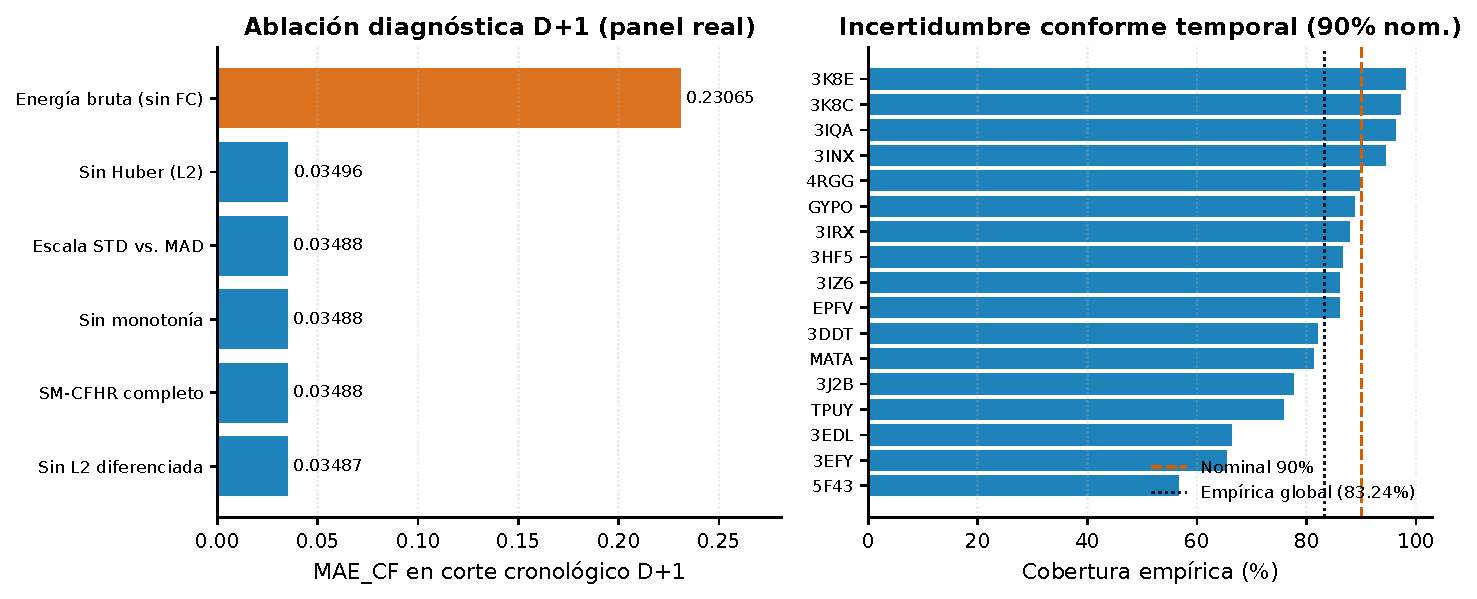
\includegraphics[width=0.98\textwidth]{figures/fig_res_oof_ablaciones_y_conformal.pdf}
\caption{Ablación diagnóstica en $D+1$ (izquierda) y cobertura empírica por central de los intervalos conformes temporales al $90\%$ nominal (derecha).}
\label{fig:res_oof_ablaciones}
\end{figure}

\subsection{Síntesis de hipótesis científicas H1--H4}

\begin{table}[!htbp]
\caption{Estado verificado de las hipótesis H1--H4 sobre las predicciones OOF congeladas y su reconciliación inferencial.}\label{tab:res_hipotesis}
\scriptsize
\setlength{\tabcolsep}{3.5pt}
\begin{tabular}{@{}p{2.3cm}p{2.7cm}p{6.5cm}@{}}
\toprule
Hipótesis & Estado verificado & Evidencia cuantitativa exacta \\
\midrule
\textbf{H1} (Normalización FC en ET) & \textbf{Respaldada solo en comparación de sistemas frente a referencias en $\text{kWh}$ (no aislada)} & En $D+1$ ET con clima logra rango $1/23$ ($-22{,}16\%$ frente a \texttt{Mejor\_Bib} en $\text{kWh}$) y en el corte único $D+1$ retirar FC multiplica el error por $4{,}45\times$; dado que las $22$ referencias operaron en energía bruta, la evidencia cerrada no aísla causalmente la normalización frente al estimador. \\
\textbf{H2} (Diferencias pareadas retrospectivas) & \textbf{Acotada a ET + Clima}; rechazada como superioridad universal & En \texttt{v1.0.3} ($T_{\mathrm{eff}} \ge 2H$): $2/15$ significativas; en el análisis retrospectivo \texttt{v2.0.0} sobre $\mathrm{MAE}_{\mathrm{macro}}$: $5/5$ en \texttt{ET + Clima} frente a \texttt{Mejor\_Bib} ($p_{\mathrm{Holm}} \le 5{,}21\times 10^{-6}$) y $45/45$ en el universo global de $252$ contrastes frente a bibliotecas ($p_{\mathrm{Holm,252}} \le 0{,}0417$), con $0$ en IP o sin clima y derrotas hasta $+24{,}24\%$ en \texttt{DirectoSinClima\_IP}. \\
\textbf{H3} (Componentes estructurales en $D+1$) & \textbf{Parcial / dependiente del corte} & La normalización FC explica la mayor caída ($4{,}45\times$); Huber aporta estabilidad bajo contaminación sintética ($10\%$); monotonía y MAD coinciden con el corte limpio sin restricción. \\
\textbf{H4} (Fixed vs.\ HPO) & \textbf{Refutada para HPO}; \texttt{Fixed} domina en precisión y coste & \texttt{Fixed} ($B=0$) supera a \texttt{HPO} ($B=25$) en $19/28$ escenarios ($14/14$ ET; $4$ victorias Holm frente a $1$ derrota) con coste $59\times$ menor. \\
\bottomrule
\end{tabular}
\end{table}

\section{Discusión}\label{sec:discusion}

Los resultados definitivos fuera de muestra permiten contrastar las decisiones de diseño de SM-CFHR frente a la evidencia empírica y delimitar con precisión dónde aporta ventaja real y dónde falla frente a alternativas locales o no lineales.

\subsection{Interpretación empírica por régimen, horizonte y estrategia}

\begin{enumerate}
    \item \textbf{Ventaja concentrada en transferencia espaciotemporal con meteorología:} la combinación de normalización causal por $24\,000\,C_{i,t}$, regularización anisotrópica y cotas monótonas logra rango $1{,}0/23$ y $5/5$ victorias Holm bajo el estimando $\mathrm{MAE}_{\mathrm{macro}}$ en \texttt{D+1 ET} y \texttt{RecGEFSv12 ET} ($7$--$28$~días). Al evaluar plantas nunca vistas durante el ajuste, los regresores entrenados en energía bruta ($\text{kWh/día}$) sufren la distorsión de escala de $39{,}6\times$, mientras SM-CFHR transfiere relaciones adimensionales consistentes entre zonas geográficas.
    \item \textbf{Limitaciones en intraplanta y caída en estrategia directa sin clima:} cuando existe historial propio de la planta (\texttt{IP}), las bibliotecas locales o flexibles (\texttt{BayesianRidge}, \texttt{k-NN}, \texttt{Random Forest}) aprovechan relaciones no lineales y niveles específicos de energía sin necesitar transferencia de escala. En particular, en \texttt{DirectoSinClima\_IP} ($7$--$28$~días), el ajuste lineal adimensional sobre acumulados sin señal NWP se degrada hasta $+24{,}24\%$ frente a \texttt{k-NN}, constituyendo un resultado negativo claro del método.
    \item \textbf{Compromiso entre configuración fija y HPO:} \texttt{SM-CFHR-Fixed} ($B=0$) supera a \texttt{SM-CFHR-HPO} ($B=25$) en $19/28$ escenarios ($14/14$ en ET; $4$ victorias Holm frente a $1$ derrota) con un coste de pared $59\times$ menor. La varianza de selección en $3$ pliegues internos penaliza a \texttt{HPO} especialmente en transferencia espacial y horizontes largos, mostrando que el sesgo inductivo fijo actúa como regularizador efectivo.
    \item \textbf{Sensibilidad de escala ($\text{kWh}$ vs.\ CF) y subcobertura conformal:} el contraste entre rango medio $2{,}93/23$ en $\text{kWh}$ y $4{,}00/23$ en $\mathrm{MAE}_{\mathrm{CF,macro}}$ evidencia que las centrales de mayor potencia influyen fuertemente en las métricas en energía absoluta. Asimismo, las coberturas conformes empíricas ($83{,}24\%$ para $90\%$ nominal; $69{,}25\%$ para $80\%$) confirman que la no estacionariedad y deriva entre bloques violan la intercambiabilidad estándar \cite{barber2023nonexchangeable}.
\end{enumerate}

\subsection{Implicaciones estructurales de las decisiones de diseño}

La arquitectura de SM-CFHR introduce cuatro sesgos inductivos explícitos: normalización causal por $24\,000\,C_{i,t}$, escalado MAD con pérdida de Huber, penalización $L_2$ anisotrópica ($\alpha_{\mathrm{lin}}, \alpha_{\mathrm{meteo}}$) y restricciones de signo no negativo sobre la persistencia reciente y la irradiación pronosticada. Esta elección privilegia la estabilidad paramétrica, la convexidad del ajuste de un paso y la invariancia de escala entre centrales de $9{,}8$ a $388{,}0$~MW, a costa de restringir la flexibilidad funcional frente a relaciones no lineales complejas entre variables meteorológicas. Asimismo, en el despliegue recursivo multihorizonte ($H \in \{7,14,21,28\}$), la realimentación de predicciones propias mediante ventana deslizante y amortiguamiento $\gamma_h = 0{,}85^{h-1}$ transforma un problema interno convexo en una composición no lineal de horizonte $H$, haciendo indispensable que la validación interna de hiperparámetros reproduzca exactamente esa misma dinámica recursiva.

En el plano experimental, cuatro aspectos condicionan la interpretación de cualquier resultado futuro: (1) la asimetría de presupuestos de búsqueda entre \texttt{SM-CFHR-Fixed} ($B=0$), los modelos de referencia (rejilla de $4$ configuraciones) y \texttt{SM-CFHR-HPO} ($B=25$ ensayos TPE), razón por la cual la comparación primaria se fija en $B=0$; (2) la reutilización adaptativa del panel histórico 2024--2026 durante el desarrollo de los modelos previos y la consolidación de SM-CFHR \cite{cawley2010overfit}; (3) el sesgo potencial de selección posterior al comparar en pruebas pareadas frente al mejor competidor de biblioteca identificado sobre la propia muestra de evaluación, que exige complementar dicho contraste con la línea base preespecificada \texttt{MM30}, comparaciones exploratorias frente a referencias individuales de biblioteca y pruebas múltiples (SPA y MCS con interpretación estricta), junto con la distinción entre la métrica física exportada en $\text{kWh/día}$ (ponderada por capacidad instalada) y métricas adimensionales en factor de capacidad ($\mathrm{MAE}_{\mathrm{CF}}$, calculable post-hoc sobre las predicciones OOF); y (4) el tamaño muestral efectivo reducido en horizontes de $21$ y $28$ días con orígenes no solapados, donde la autocorrelación residual limita la potencia de los contrastes pareados ($T_{\mathrm{eff}} < 2H$).

\subsection{Limitaciones de generalización}\label{sec:limitaciones_gen}

El estudio utiliza exclusivamente $17$ centrales fotovoltaicas de un mismo dominio geográfico y regulatorio (el Sistema Interconectado Nacional de Colombia) y no evalúa conjuntos de datos externos independientes de naturaleza distinta. Esta limitación científica exige distinguir con rigor cuatro dimensiones de generalización, ninguna de las cuales implica automáticamente a las demás:

\begin{enumerate}
    \item \textbf{Generalización espacial:} mide el desempeño sobre centrales o zonas geográficas apartadas del entrenamiento dentro de la misma cohorte colombiana mediante validación \textit{leave-one-group-out}. Aunque este protocolo evita la fuga entre plantas vecinas situadas a menos de $100\text{ km}$, la flota comprende solo $G=7$ conglomerados espaciales \cite{cameron2015cluster}, por lo que la extrapolación a regímenes climáticos distintos (como zonas desérticas extratropicales o latitudes altas con marcada estacionalidad solar) no queda demostrada.
    \item \textbf{Generalización temporal:} mide el desempeño sobre periodos no utilizados para ajustar parámetros dentro de la ventana enero de 2024--octubre de 2026. Dado que la arquitectura fue fijada tras inspeccionar la estructura exploratoria de ese mismo intervalo histórico, la evaluación OOF mide generalización temporal retrospectiva bajo particiones causales, no desempeño prospectivo sobre años futuros ni cambios estructurales de red posteriores a octubre de 2026.
    \item \textbf{Generalización entre datasets:} mide el desempeño frente a fuentes de medición, resoluciones temporales, sistemas de telemetría o procesos de generación de datos diferentes (por ejemplo, datos SCADA a nivel de inversor, otras redes eléctricas o distintas mallas NWP). Al no haberse evaluado ningún conjunto de datos externo independiente de XM/Open-Meteo/GEFSv12, no puede afirmarse invarianza frente a cambios de fuente o protocolo de registro.
    \item \textbf{Generalización entre dominios:} concierne a la transferibilidad de los principios de SM-CFHR fuera del pronóstico fotovoltaico. La normalización por $24\,000\,C_{i,t}$, el acotamiento físico al intervalo $[0,1]$, el amortiguamiento geométrico de persistencia y las restricciones de no negatividad sobre la persistencia de $30$ días y la irradiación pronosticada dependen específicamente de la física de generación solar. Su adaptación a otros dominios de regresión requeriría redefinir justificadamente las transformaciones de escala, los grupos de regularización y las restricciones de signo pertinentes; por ello, la evaluación diseñada no demuestra universalidad del estimador.
\end{enumerate}

\section{Conclusiones y disponibilidad}\label{sec:conclusiones}

Este trabajo ha formalizado el modelo \textbf{SM-CFHR} (\textit{Structured Monotone Capacity-Factor Huber Regressor}), su análisis matemático y verificación formal en Lean~4, la evaluación OOF congelada sobre $28$ configuraciones (\texttt{v1.0.3}), la reconciliación inferencial y en factor de capacidad (\texttt{v2.0.0}) y el experimento controlado de equivalencia de representación y ablación factorial (\texttt{v3.0.0}).

En el plano teórico y formal, la normalización causal por capacidad vigente al origen ($24\,000\,C_{i,t}$) unifica objetivos diarios y acumulados eliminando la heterogeneidad de $39{,}6\times$ sin fuga temporal; asimismo, el programa convexo de Huber con regularización anisotrópica y cotas de no negatividad posee existencia global, unicidad de $\mathbf{w}^*$, unicidad condicional de $b^*$ y equivalencia KKT verificadas en Lean~4 (\texttt{v4.36.0}) sobre $\mathbb{R}$ (con demostración analítica de la cota espectral completa $L_J$ en el Material Suplementario, Sección~S1).

En el plano empírico, la evidencia combinada de las tres capas del estudio permite concluir con precisión:
\begin{enumerate}
    \item \textbf{La contribución principal demostrada es la representación causal en factor de capacidad y el protocolo multihorizonte sin fuga:} al equiparar la representación a factor de capacidad en \texttt{v3.0.0}, las siete familias evaluadas mejoran entre $-10{,}13\%$ y $-23{,}24\%$ en $\mathrm{MAE}_{\mathrm{CF,macro}}$ medio, y retirar dicha normalización degrada el error en $+25{,}86\%$ de media (hasta $+62{,}65\%$).
    \item \textbf{No se demuestra superioridad algorítmica universal de SM-CFHR frente a lineales regularizados en factor de capacidad:} bajo representación equiparada, \texttt{SM-CFHR} empata o queda a $+0{,}13\%$--$+1{,}58\%$ de \texttt{BayesianRidge-CF} y \texttt{ElasticNet-CF} en transferencia espaciotemporal (ganando solo en \texttt{RecGEFSv12\_ET\_7d} en Condición~A, $-0{,}56\%$, y en \texttt{D1\_ET\_5var} en Condición~B, $-0{,}09\%$) y pierde sistemáticamente en régimen intraplanta ($+3{,}23\%$ a $+16{,}24\%$).
    \item \textbf{Los componentes secundarios aportan beneficios acotados o dependientes del régimen:} las variables NWP ($+18{,}52\%$) y anomalías ($+5{,}61\%$) son determinantes; la configuración fija ($B=0$) supera a \texttt{HPO} ($B=25$) en $19/28$ escenarios con coste $59\times$ menor; y la pérdida de Huber protege frente a contaminación severa del objetivo ($10\%$) pero no ante apalancamiento en covariables. Permanece vigente \texttt{autorizacion\_alcance\_solar\_docente: false}.
\end{enumerate}

\subsection*{Disponibilidad de código y reproducibilidad}

El código fuente del estimador, el protocolo experimental, las pruebas automatizadas, la formalización en Lean~4 y el manuscrito están disponibles para reproducción computacional \cite{peng2011reproducible} en el repositorio oficial \url{https://github.com/KrissV89/sm-cfhr} (etiqueta de publicación \texttt{v1.0.3-polyform}, protocolo científico \texttt{v1.0.3}, con huella SHA-256 verificable del núcleo matemático). El software original se distribuye bajo la licencia \textbf{PolyForm Noncommercial~1.0.0}, que permite el uso gratuito para investigación académica, estudio y reproducción científica; todo uso comercial o con ánimo de lucro requiere licencia comercial aparte (\texttt{edmolinares@soulspacers.com}). Esta licencia cubre únicamente el código original: los datos externos de XM, Open-Meteo y Global Energy Monitor mantienen sus propias condiciones de uso (por su tamaño de $603{,}70$~MB sin comprimir y restricciones de redistribución se provee un flujo de importación local y verificación SHA-256; Figura~\ref{fig:pipeline_repro}), las dependencias de terceros conservan sus respectivas licencias y el presente manuscrito junto con sus figuras mantiene sus derechos académicos independientes.

\begin{figure}[!htbp]
\centering
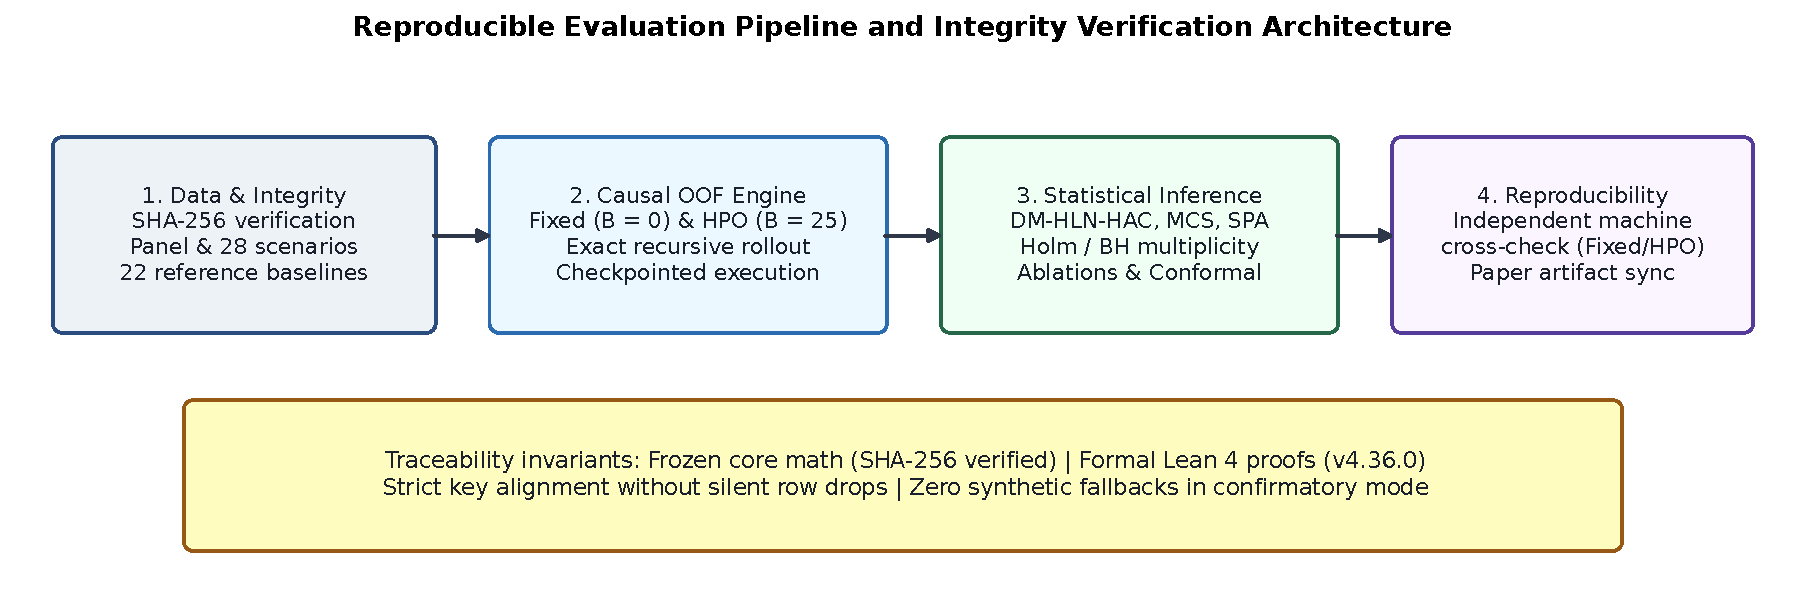
\includegraphics[width=0.98\textwidth]{figures/fig_pipeline_reproduccion.pdf}
\caption{Arquitectura de ejecución resumible, verificación de integridad mediante SHA-256 y comparación numérica entre máquinas independientes.}
\label{fig:pipeline_repro}
\end{figure}


\let\oldthebibliography\thebibliography
\renewcommand{\thebibliography}[1]{\oldthebibliography{#1}\small\setlength{\itemsep}{1pt plus 0.5pt minus 0.5pt}\setlength{\parskip}{0pt}}
\bibliography{bibliography/bibliography}

\end{document}
